\makeatletter
\def\@listi{\topsep=4pt plus 2pt   \parsep=\parskip  \partopsep=0pt plus 1pt }
\makeatother

\newcommand\BNF{\(\mathrel{\mathtt{:}}\mathrel{\mathtt{:}}=\)}
\newcommand\ALT{\(|\)}
\newcommand\TERM[1]{{\tt #1}}
\newcommand\NT[1]{{\it #1\/}}
\newcommand\GROUP[1]{\(\bigl(\)#1\(\bigr)\)}
\newcommand\OPTIONAL{{\small\(^?\)}}
\newcommand\KLEENE{\(^*\)}
\newcommand\KLEENEPLUS{\(^+\)}

  \let\1=\fortresscodeindentone
  \let\2=\fortresscodeindenttwo


\let\codeexamplesize=\small

\section{Introduction and Background}
\seclabel{introduction}


A longstanding problem with multiple inheritance is what to do when
methods inherited from several parents conflict.  This is actually
an important special case of the more general problem of
what to do when a method or function is overloaded, that is,
having multiple definitions that may arise from a variety of sources,
of which inheritance from a parent is one possibility.
Many approaches have
been explored in the literature; some unfortunately violate the
intuitively desirable requirement that, for any given invocation,
the function or method definition invoked
be the uniquely most specific one that is both accessible and
applicable.  The problem is that there might be two (or more)
accessible definitions that are applicable, equally specific,
and more specific than any of the others (in such a situation,
we say that the invocation is \emph{ambiguous}).
Many language designs solve this problem by adopting some sort of asymmetric
``tie-break'' rule that arbitrarily chooses one definition in preference to others
that are otherwise equally specific; for example, in the context of inheritance,
one might examine the textual order in which the parents are declared
and prefer definitions from parents that occur earlier (or later) in this ordering.

The Fortress programming language, on the other hand, addresses the problem by
simply prohibiting it from arising: the signatures in every overload set are
required to form a meet-bounded lattice (the ``Meet Rule''), and therefore it is impossible for any
function or method call to be ambiguous.  This idea goes back nearly two decades
to the work of
Castagna~\emph{et~al.}~\cite{LFP92-OVERLOADED-FUNCTIONS-WITH-SUBTYPING}, but
Fortress appears to be the first programming language to adopt and statically
enforce it.
Our experience is that the requirement feels natural in practice,
and static enforcement by a compiler helps to expose programming errors.
Moreover, enforcing the requirement has two major benefits:
(a) Because the lattice structure guarantees a confluence property,
there is a modular strategy for implementing dynamic multimethod dispatch
in a simple, distributed fashion.
(b) The distributed implementation of multimethod dispatch in turn
makes it easy to divide programs into components that can be separately
compiled, with full static type checking and full static enforcement
of the Meet Rule, and with fine-grained control over the export and
import of not only type declarations but also individual function
declarations and definitions.

A general issue with method inheritance is the ``super problem'': how to allow a
method that overrides an inherited method definition to invoke that overridden
method.  In the Java\texttrademark\ programming language, a method definition
(as opposed to an abstract declaration) can be inherited from at most one
parent, so it suffices to use the keyword {\tt super}:
\begin{verbatim}
class MyType extends MyFather {
  double myMethod(int a, double b) {
    return Math.sin(b) + super.myMethod(a, b);
  }
}
\end{verbatim}
But in a language that allows definitions to be inherited from multiple parents,
it is necessary to specify which definition is desired.  Rather than, say,
naming the parent from which the definition should be taken, Fortress uses the
dispatch mechanism itself to select to desired definition by allowing the
programmer to use the keyword \KWD{asif} to indicate that an expression should be assumed
to have a specified supertype of its usual ``run-time type'' for dispatch
purposes:
\begin{FortressCode}
\KWD{trait} \TYP{MyType} \KWD{extends} \lbrace\,\TYP{MyFather}, \TYP{MyMother}\,\rbrace \\
\2\+\VAR{myMethod}(a\COLON \mathbb{Z}32, b\COLON \mathbb{R}64)\COLON \mathbb{R}64 = \\
  \2\+(\sin(b) + (\KWDVAR{self} \KWD{asif} \TYP{MyMother}).\VAR{myMethod}(a, b) \\
    \3 \+- (\KWDVAR{self} \KWD{asif} \TYP{MyFather}).\VAR{myMethod}(3, b))\-\-\- \\
\KWD{end}
\end{FortressCode}

There is one more piece to the story.  The Fortress language is
designed to support many aspects of conventional mathematical notation,
and many mathematical operators such as $+$ and $\leq$ and $\cup$
and especially $\cdot$ and $\times$
have different definitions depending on the types of the arguments;
in a language with multiple dispatch, 
it is natural to define these operators as overloaded functions.
On the other hand, there is organizational value in arranging the mathematical
types into an object-oriented hierarchy, and so it would seem even more natural
to define operators as overloaded methods.  This is not a new idea,
and it leads to the so-called ``binary method problem''~\cite{BRUCE-ON-BINARY-METHODS}:
how to define a method that takes an argument of the same type
as the receiver, in such a way as to preserve subtype relationships.

Fortress provides a novel solution to the binary method problem: functional
methods, which have two distinctive characteristics: (i) a functional method may
designate any argument, not just the textually leftmost, to be treated as the
``dispatch target'' or ``receiver''; (ii) functional methods are inherited like conventional
``dotted methods'' but overloaded like top-level functions.  Because they are
overloaded like top-level functions, the programmer can use the component system
to exercise the same fine-grained control over export and import of individual
functional method declarations and definitions.  (For this reason, and because
they address the binary method problem nicely, we often find ourselves
preferring functional methods to dotted methods.)

Our purpose here is to explain the Fortress type system, the Meet Rule, the Fortress component system,
the \KWD{asif} keyword,
and Fortress functional methods, and then to illuminate how they interact to solve the problems of method ambiguity,
binary methods, super invocation, fine-grained namespace control, and separate compilation.

The specific novel contribution of this work is to present a strategy for implementing symmetric multimethod dispatch
in a statically typed language in which the program can be divided
into components that can be separately type-checked and separately compiled,
{\it such that the components provide complete namespace control over \underline{all} top-level names and definitions};
names of not only traits and objects, but also variables and functions and functional methods, and even individual definitions, may be selectively exported, imported, and renamed;
the Meet Rule makes possible a distributed implementation of multimethod dispatch that enables separate compilation.
The strategy is presented as a multiphase rewriting process; the source language is
a stripped-down version of Fortress, and the target language
is similar to, but simpler than, the Java programming language and is readily
supported by the Java Virtual Machine.  The demonstrated rewriting strategy is
a practical basis for separate compilation and is easily extended to
explicitly type-parameterized methods and functions.
We also comment on opportunities for optimizing the resulting target-language code.



\section{Source Language Characteristics}

The Fortress programming language integrates traditional mathematical
notation into an object-oriented framework based on traits with
multiple inheritance, overloading (of both methods and functions)
resolved by symmetric dynamic dispatch, static types, and separately
compiled modules.  An innovation of particular interest is
\emph{functional methods}, which (like conventional ``dotted methods'')
are declared within traits and may be inherited, but are invoked by
ordinary function calls (or mathematical operator syntax) rather
than conventional ``dotted method calls,'' and therefore compete
in overloading resolution with ordinary function declarations.
A component/API system governs visibility of traits, objects,
functions, and variables, but when a function definition is invoked,
it is desirable to regard overriding functions and
methods that are visible to the callee as part of its implementation,
even though they may not be visible to the caller.
We elaborate on all these points in the following subsections.

\subsection{Traits, Objects, Methods, and Functions}

Fortress organizes objects into a multiple-inheritance hierarchy based
on {\it traits}~\cite{traits,traitsOOPSLA04}.  It may be helpful for the reader familiar with the Java language~\cite{JLS1}
to think of a Fortress trait as a Java interface that can
also contain concrete method definitions, and
to think of a Fortress object declaration as a Java final class.
Fortress objects inherit only from traits, not other objects,
and fields are not inherited.  Both traits and objects may contain
(concrete) method definitions, and may inherit method definitions
from multiple supertraits (traits that they \emph{extend}).
Traits may also contain (abstract) method declarations, which impose
upon objects that inherit them (directly or indirectly)
the requirement to provide matching concrete definitions.
Thus all traits and objects form a multiple inheritance hierarchy,
a partial order defined by the \KWD{extends} relationship,
in which all objects are at the leaves.  As in the Java language and similar object-oriented
languages that have static type systems, the name of a trait or object
serves to name a type, which is the set of all objects at or below
the named position in the trait hierarchy.  In addition to objects
(all of which are of type \TYP{Object}, as in the Java language), Fortress has
\emph{arrow types} \EXP{D\rightarrow{}R} (the types of functions) and \emph{tuples}
written as \EXP{(e_1, e_2, \ldots, e_{n})} whose types form a partial order
in the usual conjunctive elementwise manner:
\EXP{(T_{1}, T_{2}, \ldots, T_{m}) \unlhd (U_{1}, U_{2}, \mathinner{\ldotp\ldotp}, U_{n})} if and only if
\EXP{m=n} and, for all \EXP{1\leq{}k\leq{}m}, \EXP{T_{k} \unlhd U_{k}}.  Objects, functions, and tuples
are all \emph{values} and have type \TYP{Any}.

Like C++~\cite{C-PLUS-PLUS} (and unlike the Java language~\cite{JLS1}
and C\#~\cite{CSHARP-ECMA-334-2001}), Fortress provides not
only methods associated with objects but also functions not associated with
any object; moreover, Fortress function definitions and declarations may be either
top-level or local to a block.  (We use the term
\emph{definition} to refer to a syntactic construct that defines a variable, function,
or method, and furthermore contains an executable expression to supply
the value of the variable, invoked function, or invoked method.
The term \emph{declaration} applies whether or not such an expression is present.)

As in many previous languages, both functions and methods may be
\emph{overloaded}; that is, there may be many methods within an
object, or many functions declared within the same scope, that have
the same name.  This raises the issue of \emph{overload resolution}:
given a method call or function call, how does the language determine
which definition(s) should be invoked?  If a single
definition is to be chosen and invoked, then we call this determination
process the \emph{dispatch mechanism}.  A typical dispatch mechanism
identifies a pool of candidate definitions that are \emph{accessible}
and \emph{applicable}, then selects from that pool the one that is
\emph{most specific}.  Many dispatch mechanisms have
been explored in the literature, and they differ in their definitions
of ``accessible'' and ``applicable'' and ``most specific'';
in particular, they may differ in whether static type information,
dynamic (run-time) information about the arguments, or both are
brought to bear in defining each of these three terms.
If static information is used, then the dispatch mechanism may
have two stages, one performed at some time prior to program
execution (such as compile time) and one performed during program
execution.
For example, the Java language uses a \emph{single dynamic dispatch} mechanism
for method calls,
in which both static and dynamic information about the receiver
object is used but only static information about the other arguments
is used; a method signature is chosen at compile time based on all
the static information, and further dispatch occurs at run time
based on the actual class of the receiver object (which may turn out to be
more specific than the static type of the receiver object expression).
As another example, the Common Lisp Object System (CLOS)~\cite{ECOOP87-CLOS,CLOS-SPECIFICATION,CLTL2,CACM-CLOS}
performs \emph{asymmetric multiple dynamic dispatch}
in which only dynamic information is used, but for all arguments,
not just one designated ``receiver'' argument.
(While Common Lisp used the term ``generic function,'' nowadays
that term is usually used to refer to a function that is polymorphic
by virtue of having explicit static type parameters, and
the term \emph{multimethod} is used to refer to a set of methods
with a dispatch discipline that takes into account dynamic information
from more than one argument.)
While CLOS performs dynamic dispatch on all arguments,
the arguments are treated asymmetrically in that the most specific
method is chosen by testing the parameter types of the candidate
methods in a specific order (normally left-to-right, though this order
can be modified for a particular overload set by an explicit declaration).
In contrast, Fortress has the behavior of \emph{symmetric multiple dynamic dispatch}:
the method ultimately chosen depends on the ilks of \emph{all} the arguments.
(We use the term \emph{ilk} for what is sometimes confusingly called a ``run-time type'';
just as the Java language has had the slogan ``Variables have types, objects have classes'' \cite[\S 4.5.5]{JLS1}
so Fortress has the slogan ``Expressions have types, values have ilks.''
Among all the types to which a given object might belong, its ilk
is (necessarily) the most specific.)
However, Fortress also makes use of static type information to perform part of the
dispatch at compile time, so it has a two-stage dispatch process.
(As we will see, this two-stage process is designed to have
the same behavior as a single-stage, fully dynamic dispatch,
so the use of static information serves purely as a performance optimization.)
Moreover, which methods are accessible depends in part
on visibility constraints that may be imposed by dividing a program
into components (see \secref{intro-components}).
One goal of this paper is to illuminate all these details.

Languages also differ in whether a method or function call can be \emph{ambiguous}
in the presence of overloading, and in how ambiguity is detected and handled.
Assume that {\tt String} is a subtype of {\tt Object}.
In the Java language, for example, one may declare two methods as follows:
\begin{tabbing}
{\tt int gnard(a:~String, b:~Object) \{ return 1; \}} \\
{\tt int gnard(a:~Object, b:~String) \{ return 2; \}}
\end{tabbing}
Whatever the type of the receiver object {\tt x},
we may observe that a method call {\tt x.gnard("foo", "quux")}
having two strings as arguments will be ambiguous, because both methods
are applicable and neither is more specific than the other.  As another example,
consider three Java interfaces named {\tt A}, {\tt B}, and {\tt C}---where
{\tt C} extends both {\tt A} and {\tt B}---and then consider these three methods
occurring in some class:
\begin{tabbing}
{\tt void zam(p: C) \{ System.out.println(jax(p)); \}} \\
{\tt int jax(q: A) \{ return 1; \}} \\
{\tt int jax(q: B) \{ return 2; \}}
\end{tabbing}
Although the Java language does not have multiple inheritance, it does have multiple
supertypes (through the interface hierarchy), and this allows the
construction of a method call {\tt jax(p)} that is type-correct but ambiguous.
{\it The Java Language Specification}~\cite[\S 15.11.2.2]{JLS1} stipulates that it is permissible
to declare such sets of methods, but it is a static error for a program
to contain a method call that will be ambiguous in their presence.
In contrast, Fortress stipulates that an ambiguous set of overloaded method or function
declarations in itself constitutes a static error, even if no call to such a method
or function appears in the program.

There is yet another distinction to be made:
some languages with multiple inheritance, such as MultiJava~\cite{MULTIJAVA-OOPSLA-2000,MULTIJAVA-TOPLAS-2006}
and Scala~\cite{SCALA-ABSTRACTIONS},
have \emph{asymmetric inheritance}, in which one superclass or supertrait
may be treated differently from another based on a criterion such
as order of declaration, and this asymmetric treatment may affect
the definition of which method is considered ``most specific''
by the dispatch mechanism (for example, ties might be broken by
choosing the method inherited from the supertrait declared earlier).
Fortress, in contrast, uses \emph{symmetric inheritance}; methods are inherited
on an equal footing from all supertraits.  This is another possible source
of method ambiguity: two methods with apparently identical signatures
may be inherited from two different supertraits.  For example,
suppose that we have three Fortress traits as follows:
\begin{codeexamplesize}
\begin{tabbing}
\EXP{\KWD{trait} \mathrm{C} \KWD{extends} \lbrace\,\mathrm{A}, \mathrm{B}\,\rbrace} \\
\(\2\)\EXP{\VAR{zam}(\ultrathin)\COLON (\ultrathin) = \VAR{println}\bigl(\KWDVAR{self}.\VAR{jax}(\ultrathin)\bigr)} \\
\EXP{\KWD{end}} \\[6pt]
\EXP{\KWD{trait} \mathrm{A}} \\
\(\2\)\EXP{\VAR{jax}(\ultrathin)\COLON \mathbb{Z}32 = 1} \fortresscommentsep \fortresslinecomment{ \EXP{\mathbb{Z}32} is the type of 32-bit integers}\\
\EXP{\KWD{end}} \\[6pt]
\EXP{\KWD{trait} \mathrm{B}} \\
\(\2\)\EXP{\VAR{jax}(\ultrathin)\COLON \mathbb{Z}32 = 2} \\
\EXP{\KWD{end}}
\end{tabbing}
\end{codeexamplesize}
This is similar to the previous example.  Because definitions of method \VAR{jax} are
inherited symmetrically by trait \EXP{\mathrm{C}}, it's a tie: it is not clear which one should be invoked
by the method call \EXP{\KWDVAR{self}.\VAR{jax}(\ultrathin)} in method \VAR{zam}.  (By the way, \EXP{\KWDVAR{self}.\VAR{jax}(\ultrathin)} could
have been written more succinctly as simply \EXP{\VAR{jax}(\ultrathin)}, just as in the Java language; we chose the longer
form for this example for the sake of clarity.)  So this example is a static error
in Fortress and will be rejected by the compiler (indeed, it would be rejected even
if the method definition for \VAR{zam} were removed).

Fortress stipulates that such ties must be broken by the programmer.
Following Castagna~\emph{et~al.}~\cite{LFP92-OVERLOADED-FUNCTIONS-WITH-SUBTYPING}, Fortress requires that the signatures
of all the functions or methods in an overload set form a \emph{meet-bounded lattice}---we call this the Meet Rule.
Simply put, for every pair of accessible signatures for which it might be possible
to construct an ambiguous call (that is, both are applicable and neither is more specific
than the other), there must be a third accessible signature that (a) is more
specific than each of the other two signatures, and (b) is also applicable to the call, and therefore will
be chosen unambiguously over the other two.
We can repair the previous example by introducing an appropriate definition of \VAR{jax} into trait \EXP{\mathrm{C}}.
This might simply supply a value on its own:
\begin{codeexamplesize}
\begin{tabbing}
%\EXP{\KWD{trait}\; \mathrm{C}\; \KWD{extends} \lbrace\,\mathrm{A}, \mathrm{B}\,\rbrace} \\
%\(\2\)\EXP{\VAR{zam}(\ultrathin)\COLON (\ultrathin) = \VAR{println}\bigl(\KWDVAR{self}.\VAR{jax}(\ultrathin)\bigr)} \\
\(\2\)\EXP{\VAR{jax}(\ultrathin)\COLON \mathbb{Z}32 = 47}
%\\
%\EXP{\KWD{end}}
\end{tabbing}
\end{codeexamplesize}
or choose to direct control to one of the inherited definitions:
\begin{codeexamplesize}
\begin{tabbing}
%\EXP{\KWD{trait}\; \mathrm{C}\; \KWD{extends} \lbrace\,\mathrm{A}, \mathrm{B}\,\rbrace} \\
%\(\2\)\EXP{\VAR{zam}(\ultrathin)\COLON (\ultrathin) = \VAR{println}\bigl(\KWDVAR{self}.\VAR{jax}(\ultrathin)\bigr)} \\
\(\2\)\EXP{\VAR{jax}(\ultrathin)\COLON \mathbb{Z}32 = (\KWDVAR{self} \KWD{asif} \mathrm{B}).\VAR{jax}(\ultrathin)} 
%\\
%\EXP{\KWD{end}}
\end{tabbing}
\end{codeexamplesize}
or might even use more than one of the inherited definitions:
\begin{codeexamplesize}
\begin{tabbing}
%\EXP{\KWD{trait}\; \mathrm{C}\; \KWD{extends} \lbrace\,\mathrm{A}, \mathrm{B}\,\rbrace} \\
%\(\2\)\EXP{\VAR{zam}(\ultrathin)\COLON (\ultrathin) = \VAR{println}\bigl(\KWDVAR{self}.\VAR{jax}(\ultrathin)\bigr)} \\
\(\2\)\EXP{\VAR{jax}(\ultrathin)\COLON \mathbb{Z}32 = (\KWDVAR{self} \KWD{asif} \mathrm{A}).\VAR{jax}(\ultrathin) + (\KWDVAR{self} \KWD{asif} \mathrm{B}).\VAR{jax}(\ultrathin)} 
%\\
%\EXP{\KWD{end}}
\end{tabbing}
\end{codeexamplesize}
(As we shall see, the Fortress \KWD{asif} construction addresses the same issues that {\tt super} does in the Java language.)

In addition to the Meet Rule, Fortress imposes the usual Result Subtype Rule:
for any pair of accessible functions or methods in an overload set, if the first
is more specific than the second, then the result type of the first
must be a subtype of the result type of the second.  This rule is necessary
to maintain type soundness.

Fortress also has parametric polymorphism of traits, objects, methods, and functions;
any of these may have static type parameters, and references to them may supply explicit
static arguments, which may be types, boolean values, integers, or operator symbols.
However, we do not address parametric polymorphism of traits and objects in this paper,
and we discuss parametric polymorphism of functions and methods only
briefly, in \secref{polymorphism}.

\subsection{Functional Methods}

As the Fortress design team has previously reported~\cite{FORTRESS-MODULAR-MULTIPLE-DISPATCH},
Fortress has not only \emph{dotted methods} that
are declared much as in the Java language and are invoked with a 
\emph{dotted method call} of the form:
\begin{codeexamplesize}
\begin{tabbing}
\EXP{\VAR{receiver}.\VAR{methodName}(e_{1}, e_{2}, \ldots, e_{n})}
\end{tabbing}
\end{codeexamplesize}
but also \emph{functional methods}.  The declaration
of a functional method differs from that of a dotted method
in that exactly one of the parameter \EXP{\VAR{name}\COLON \TYP{Type}} declarations
in the header is replaced with the keyword \EXP{\KWDVAR{self}}; in effect,
that argument position, rather than a separate expression
``before the dot,'' is treated as the receiver.
This feature easily solves the ``binary method problem'' \cite{BRUCE-ON-BINARY-METHODS}:
Suppose that we define a trait \TYP{Point} having real-valued fields \VAR{x} and \VAR{y} and a method that tests equality
of points by comparing their \VAR{x} and \VAR{y} components:
\begin{codeexamplesize}
\begin{FortressCode}
\KWD{trait} \TYP{Point} \\
\2\+x\COLON \mathbb{R} \\
  y\COLON \mathbb{R} \\
  \VAR{equal}(\KWDVAR{self}, \VAR{other}\COLON \TYP{Point})\COLON \TYP{Boolean} = \\
  \2\+(x = \VAR{other}.x) \wedge (y = \VAR{other}.y)\-\- \\
\KWD{end}
\end{FortressCode}
\end{codeexamplesize}
(In Fortress, traits cannot really have fields, but the field declaration syntax
is construed as implicitly declaring abstract getter methods:
\begin{codeexamplesize}
\begin{FortressCode}
{\tt ~~}\+\KWD{getter} x(\ultrathin)\COLON \mathbb{R} \\
  \KWD{getter} y(\ultrathin)\COLON \mathbb{R}\-
\end{FortressCode}
\end{codeexamplesize}
and a field access expression such as \EXP{p.x} is construed to mean \EXP{p.x(\ultrathin)}
if \VAR{x} names a getter method.  Field declarations in objects,
as opposed to traits, \emph{do} declare actual fields, and furthermore
implicitly declare concrete getter methods that will fetch the values of
those fields.)

Now we wish to extend this trait to create a new trait \TYP{ColorPoint}
that has an additional field \VAR{c} of type \TYP{Color}, and we ask that equality comparison
of colored points should also test whether they have the same color.
We may write:
\begin{codeexamplesize}
\begin{FortressCode}
\KWD{trait} \TYP{ColorPoint} \KWD{extends} \TYP{Point} \\
\2\+c\COLON \TYP{Color} \\
  \VAR{equal}(\KWDVAR{self}, \VAR{other}\COLON \TYP{ColorPoint})\COLON \TYP{Boolean} = \\
  \2\+(x = \VAR{other}.x) \wedge (y = \VAR{other}.y) \wedge (c = \VAR{other}.c)\-\- \\
\KWD{end}
\end{FortressCode}
\end{codeexamplesize}
There are now two points to observe.  First: \TYP{ColorPoint} is not only
a subtrait of \TYP{Point} but in fact a subtype of \TYP{Point}.  In Fortress,
subtraits are always subtypes because of various constraints in the language
specification as to what programs are valid, but we say this explicitly
because in the example language of Bruce~et~al.~\cite{BRUCE-ON-BINARY-METHODS}
subclasses are not necessarily subtypes---indeed, they were exploring the
very question of what constraints are necessary for a subclass to be a subtype.
In this example, unlike that in section~2.1 of Bruce~et~al.,
\TYP{ColorPoint} not only provides an explicit definition of method \VAR{equal}
but also inherits a definition of method \VAR{equal} from \TYP{Point}, just as it inherits
the abstract getter methods for \VAR{x} and \VAR{y} (and therefore any object that
extends \TYP{ColorPoint} inherits an obligation to implement those getter methods,
as well as inheriting the obligation to implement a getter method for \VAR{c}).
As a result, the functional method \VAR{equal} may correctly be called with
any mixture of \TYP{Point} and \TYP{ColorPoint} arguments; if both arguments are
colored points, then the definition in \TYP{ColorPoint} will be used,
and otherwise the definition in \TYP{Point} will be used.
Therefore Fortress solves the classic \TYP{ColorPoint} ``binary method problem''
as presented in Bruce~et~al.

Second: Using the definitions just shown,
\EXP{\VAR{equal}(p,\VAR{cp})} simply ignores the color of \VAR{cp} when
comparing point \VAR{p} to colored point \VAR{cp}.
We might want to control this behavior more finely by providing
explicit method definitions for
the cases where a point is compared with a colored point---for example,
to treat an ordinary point as if its color were \TYP{Purple}.
We might try using functional methods this way,
without having to modify the definition of \TYP{Point}:
\begin{codeexamplesize}
\begin{FortressCode}
\KWD{trait} \TYP{ColorPoint} \KWD{extends} \TYP{Point}\fortresscommentsep   \*{ incorrect example} \\
\2\+c\COLON \TYP{Color} \\
  \VAR{equal}(\KWDVAR{self}, \VAR{other}\COLON \TYP{ColorPoint})\COLON \TYP{Boolean} = \\
  \2\+(x = \VAR{other}.x) \wedge (y = \VAR{other}.y) \wedge (c = \VAR{other}.c)\- \\
  \VAR{equal}(\KWDVAR{self}, \VAR{other}\COLON \TYP{Point})\COLON \TYP{Boolean} = \\
  \2\+(x = \VAR{other}.x) \wedge (y = \VAR{other}.y) \wedge (c = \TYP{Purple})\- \\
  \VAR{equal}(\VAR{other}\COLON \TYP{Point}, \KWDVAR{self})\COLON \TYP{Boolean} = \VAR{equal}(\KWDVAR{self}, \VAR{other})\- \\
\KWD{end}
\end{FortressCode}
\end{codeexamplesize}
The third definition of \VAR{equal} in \TYP{ColorPoint}
has the \EXP{\KWDVAR{self}} keyword in the second parameter position,
and therefore is considered applicable to invocations that have
an argument of type \TYP{ColoredPoint} in the second argument position
(and an argument of type \TYP{Point} in the first position)---so far, so good.
The problem is that the Meet Rule in Fortress must statically forbid overloadings
in which there are two functional methods, neither more specific than the other
and neither excluding the other, in which the \EXP{\KWDVAR{self}} parameter appears in different
argument positions.  (The problem is that the compiler needs to decide statically
which argument position to treat as the receiver, without knowing the precise set
of dynamically available overloadings.)  As a result, the current design of
Fortress does \emph{not} solve this particular extended version of the binary method
problem, and we regard this as an area for future research.

We furthermore observe that other traits, completely unrelated to points
and colored points, might also define functional methods
named \VAR{equal}, and there might also be top-level
definitions of functions named \VAR{equal}.  All these constitute
one large overload set, and as long as the Meet Rule
and the Result Subtype Rule (governing consistency of return types
when one definition is more specific than another) are satisfied,
overloading ambiguity will not occur.

To guarantee this lack of ambiguity, sometimes it is necessary
to declare that two traits \emph{exclude}
each other---that is, no object can belong to both traits).
To see this, consider the example that originally motivated
the introduction of functional methods into Fortress.
We have a \TYP{Vector} trait that implements typical mathematical vector operations
such as scalar multiplication, dot product, and cross product:
% \footnote{\relax
% It is (slightly) beyond the scope of
% this paper to explain the details of how the \VAR{multiply} functional methods
% can instead be defined as an \emph{operator functional methods} for operators
% such as \EXP{\cdot} and \EXP{\times}, which can be invoked by such expressions as \EXP{\mathbf{v} \cdot \mathbf{w}}
% and \EXP{\mathbf{v} \times \mathbf{w}}, and especially the
% \emph{juxtaposition operator} that allows a scalar-vector product to be written as
% simply \EXP{3\, \mathbf{w}} or a vector-matrix product as simply \EXP{\mathbf{w}\, \mathbf{A}}.  We content ourselves
% with simply presenting these alternate versions of \TYP{Vector} and \TYP{Matrix}:
% \begin{tabbing}
% \EXP{\KWD{trait} \TYP{Vector}} \\
% \(\2\)\EXP{\KWD{opr}\,\KWD{juxtaposition}(v\COLON \mathbb{R}, \KWDVAR{self})\COLON \TYP{Vector} = \ldots} \\
% \(\2\)\EXP{\KWD{opr}\, \mathord{\cdot}(\KWDVAR{self}, v\COLON \TYP{Vector})\COLON \mathbb{R} = \ldots} \\
% \(\2\)\EXP{\KWD{opr}\, \mathord{\times}(v\COLON \TYP{Vector}, \KWDVAR{self})\COLON \TYP{Vector} = \ldots} \\
% \EXP{\KWD{end}} \\[6pt]
% \EXP{\KWD{trait} \TYP{Matrix} \KWD{excludes} \lbrace\,\TYP{Vector}\,\rbrace} \\
% \(\2\)\EXP{\KWD{opr}\,\KWD{juxtaposition}(v\COLON \mathbb{R}, \KWDVAR{self})\COLON \TYP{Matrix} = \ldots} \\
% \(\2\)\EXP{\KWD{opr}\,\KWD{juxtaposition}(\KWDVAR{self}, v\COLON \TYP{Matrix})\COLON \TYP{Matrix} = \ldots} \\
% \(\2\)\EXP{\KWD{opr}\,\KWD{juxtaposition}(\KWDVAR{self}, v\COLON \TYP{Vector})\COLON \TYP{Vector} = \ldots} \\
% \(\2\)\EXP{\KWD{opr}\,\KWD{juxtaposition}(v\COLON \TYP{Vector}, \KWDVAR{self})\COLON \TYP{Vector} = \ldots} \\
% \EXP{\KWD{end}}
% \end{tabbing}
% }
\begin{codeexamplesize}
\begin{tabbing}
\EXP{\KWD{trait} \TYP{Vector}} \\
\(\2\)\EXP{\VAR{multiply}(v\COLON \mathbb{R}, \KWDVAR{self})\COLON \TYP{Vector} = \ldots} \\
\(\2\)\EXP{\VAR{dotProduct}(\KWDVAR{self}, v\COLON \TYP{Vector})\COLON \mathbb{R} = \ldots} \\
\(\2\)\EXP{\VAR{crossProduct}(v\COLON \TYP{Vector}, \KWDVAR{self})\COLON \TYP{Vector} = \ldots} \\
\EXP{\KWD{end}}
\end{tabbing}
\end{codeexamplesize}
Now we wish to define a \TYP{Matrix} trait that implements not only
scalar-matrix multiplication and
matrix-matrix multiplication but also matrix-vector multiplication and vector-matrix multiplication,
all without modifying the existing \TYP{Vector} trait.  Moreover,
unlike the example of \TYP{Point} and \TYP{ColorPoint}, it is not
appropriate for \TYP{Matrix} to be a subtrait of \TYP{Vector}.
If we simply write:
\begin{codeexamplesize}
\begin{tabbing}
\EXP{\KWD{trait} \TYP{Matrix}} \\
\(\2\)\EXP{\VAR{multiply}(v\COLON \mathbb{R}, \KWDVAR{self})\COLON \TYP{Matrix} = \ldots} \\
\(\2\)\EXP{\VAR{multiply}(\KWDVAR{self}, v\COLON \TYP{Matrix})\COLON \TYP{Matrix} = \ldots} \\
\(\2\)\EXP{\VAR{multiply}(\KWDVAR{self}, v\COLON \TYP{Vector})\COLON \TYP{Vector} = \ldots} \\
\(\2\)\EXP{\VAR{multiply}(v\COLON \TYP{Vector}, \KWDVAR{self})\COLON \TYP{Vector} = \ldots} \\
\EXP{\KWD{end}}
\end{tabbing}
\end{codeexamplesize}
the Meet Rule is not satisfied, because it is possible that some object \VAR{vm} might extend
both \TYP{Vector} and \TYP{Matrix}, and then the invocation \EXP{\VAR{multiply}(4,\VAR{vm})} would be ambiguous
because two definitions of scalar multiplication would apply, neither more specific than
the other.  A solution is to declare that \TYP{Matrix} excludes \TYP{Vector},
so that no such object can exist:
\begin{codeexamplesize}
\begin{tabbing}
\EXP{\KWD{trait} \TYP{Matrix} \KWD{excludes} \lbrace\,\TYP{Vector}\,\rbrace} \\
\(\2\)\EXP{\VAR{multiply}(v\COLON \mathbb{R}, \KWDVAR{self})\COLON \TYP{Matrix} = \ldots} \\
\(\2\)\EXP{\VAR{multiply}(\KWDVAR{self}, v\COLON \TYP{Matrix})\COLON \TYP{Matrix} = \ldots} \\
\(\2\)\EXP{\VAR{multiply}(\KWDVAR{self}, v\COLON \TYP{Vector})\COLON \TYP{Vector} = \ldots} \\
\(\2\)\EXP{\VAR{multiply}(v\COLON \TYP{Vector}, \KWDVAR{self})\COLON \TYP{Vector} = \ldots} \\
\EXP{\KWD{end}}
\end{tabbing}
\end{codeexamplesize}
Thus, while Fortress cannot currently solve the extended \TYP{ColorPoint}
example (because \TYP{ColorPoint} inherits from \TYP{Point} and therefore does
not exclude it), it handles the \TYP{Vector}/\TYP{Matrix} version of the
binary method problem quite nicely (because \TYP{Matrix} excludes \TYP{Vector}).
This suggests a partial solution to the extended \TYP{ColorPoint} problem:
if we know about a particular other trait, say \TYP{InvisiblePoint},
that extends \TYP{Point}, and is known not to have any instances in
common with \TYP{ColorPoint}, then we can write \VAR{equal} methods in \TYP{ColorPoint}
to handle all comparisons with \TYP{InvisiblePoint} without having to modify \TYP{InvisiblePoint}:
\begin{codeexamplesize}
\begin{FortressCode}
\KWD{trait} \TYP{ColorPoint} \KWD{extends} \TYP{Point} \KWD{excludes} \lbrace\,\TYP{InvisiblePoint}\,\rbrace \\
\2\+c\COLON \TYP{Color} \\
  \VAR{equal}(\KWDVAR{self}, \VAR{other}\COLON \TYP{ColorPoint})\COLON \TYP{Boolean} = \\
  \2\+(x = \VAR{other}.x) \wedge (y = \VAR{other}.y) \wedge (c = \VAR{other}.c)\- \\
  \VAR{equal}(\KWDVAR{self}, \VAR{other}\COLON \TYP{InvisiblePoint})\COLON \TYP{Boolean} = \\
  \2\+(x = \VAR{other}.x) \wedge (y = \VAR{other}.y) \wedge (c = \TYP{Purple})\- \\
  \VAR{equal}(\VAR{other}\COLON \TYP{InvisiblePoint}, \KWDVAR{self})\COLON \TYP{Boolean} = \\
  \2\+\VAR{equal}(\KWDVAR{self}, \VAR{other})\-\- \\
\KWD{end}
\end{FortressCode}
\end{codeexamplesize}
This overloading of \VAR{equal} satisfies the Meet Rule because the signature
\EXP{(\TYP{ColorPoint},\TYP{InvisiblePoint})} and the signature \EXP{(\TYP{InvisiblePoint},\TYP{ColorPoint})} exclude
each other.

In our early report \cite{FORTRESS-MODULAR-MULTIPLE-DISPATCH}, Fortress allowed functions to be overloaded with other
functions and functional methods to be overloaded with other functional methods.
Since then Fortress has been changed to allow functions and functional
methods to participate in the same overload set.  One goal of this paper
is to explain exactly how that works.  A necessary restriction is that
there must not be any top-level function
whose signature is more specific than that of a functional method
within the same overload set.

\subsection{Components and APIs}
\seclabel{intro-components}

Just as the Java language allows a program to be divided into \emph{compilation units}
that can be separately compiled, and also has \emph{packages} that provide
a modicum of namespace control, Fortress allows a program to be divided
into \emph{components}.  Interfaces between components are described
by \emph{APIs}.  Code in one component cannot refer directly to code
in another component; rather, any component or API can \emph{import}
identifiers from one or more APIs, and any component can \emph{export}
one or more APIs.  Each API must be exported by exactly one component.

Fortress also has mechanisms for bundling a set of components into
a single larger component, and this process may be carried out recursively,
thus providing namespace control for the names of components and APIs.
The details of this are beyond the scope of this paper; here we will simply
assume that the names of all components are distinct and the names
of all APIs are distinct (but the name of a component may be the same
as the name of an API).

One goal of this paper is to explain how overload sets and overload
resolution interact with the namespace control imposed by components
and APIs in Fortress.

A Fortress API can contain declarations of top-level variables,
top-level functions, traits, and objects; trait and object
definitions may contain (abstract) declarations of fields,
dotted methods, and functional methods.  Here is a simple example
of an API:
\begin{codeexamplesize}
\begin{FortressCode}
\KWD{api} \TYP{Geometry} \\
 \\
\KWD{trait} \TYP{Point} \\
\2\+x\COLON \mathbb{R} \\
  y\COLON \mathbb{R} \\
  \VAR{equal}(\KWDVAR{self}, \VAR{other}\COLON \TYP{Point})\COLON \TYP{Boolean}\- \\
\KWD{end} \\
 \\
\VAR{makePoint}(x\COLON \mathbb{R}, y\COLON \mathbb{R})\COLON \TYP{Point} \\
 \\
\KWD{end} \TYP{Geometry}
\end{FortressCode}
\end{codeexamplesize}

An API may be implemented by one or more components, but only one implementation
may be used in any given complete program.  Here is a possible implementation of
the \TYP{Geometry} API:
\begin{codeexamplesize}
\begin{FortressCode}
\KWD{component} \TYP{QuuxGeometry} \\
\KWD{export} \TYP{Geometry} \\
 \\
\KWD{trait} \TYP{Point} \\
\2\+x\COLON \mathbb{R} \\
  y\COLON \mathbb{R} \\
  \VAR{equal}(\KWDVAR{self}, \VAR{other}\COLON \TYP{Point})\COLON \TYP{Boolean} = \\
  \2\+(x = \VAR{other}.x) \wedge (y = \VAR{other}.y)\-\- \\
\KWD{end} \\
 \\
\VAR{makePoint}(x\COLON \mathbb{R}, y\COLON \mathbb{R}) = \TYP{CartesianPoint}(x, y) \\
 \\
\KWD{object} \TYP{CartesianPoint}(x\COLON \mathbb{R}, y\COLON \mathbb{R}) \KWD{extends} \TYP{Point} \KWD{end} \\
 \\
\KWD{object} \TYP{PolarPoint}(\rho\COLON \mathbb{R}, \theta\COLON \mathbb{R}) \KWD{extends} \TYP{Point} \\
\2\+\KWD{getter} x(\ultrathin) = \rho\, \cos\, \theta \\
  \KWD{getter} y(\ultrathin) = \rho\, \sin\, \theta\- \\
\KWD{end} \\
 \\
\KWD{end} \TYP{QuuxGeometry}
\end{FortressCode}
\end{codeexamplesize}
Note that \EXP{\rho} and \EXP{\theta} are legitimate identifiers in Fortress,
as they are (in principle) in the Java language.  The object
\TYP{PolarPoint} is not exported through the \TYP{Geometry}, but could be
exported as part of another API or used as part of the internal
workings of the component (not shown).


We might then have another component that can be run as a ``main program''
(because it exports the API \TYP{Executable}, which declares a top-level
function named \VAR{run}), which also imports \TYP{Color} and the
names of three colors from \TYP{ColorPackage} (not shown)
and imports ``whatever is needed'' (the ellipsis \EXP{\ldots} in the \KWD{import} statement
is actually part of Fortress ``import on demand'' syntax) from the \TYP{Geometry} API:
\begin{codeexamplesize}
\begin{FortressCode}
\KWD{component} \TYP{MyProgram} \\
\KWD{import} \TYP{ColorPackage}.\lbrace\,\TYP{Color}, \TYP{Orange}, \TYP{Green}, \TYP{Purple}\,\rbrace \\
\KWD{import} \TYP{Geometry}.\lbrace\,\ldots\,\rbrace \\
\KWD{export} \TYP{Executable} \\
 \\
\KWD{trait} \TYP{ColorPoint} \KWD{extends} \TYP{Point} \\
\2\+c\COLON \TYP{Color} \\
  \VAR{equal}(\KWDVAR{self}, \VAR{other}\COLON \TYP{ColorPoint})\COLON \TYP{Boolean} = \\
  \2\+(x = \VAR{other}.x) \wedge (y = \VAR{other}.y) \wedge (c = \VAR{other}.c)\- \\
  \VAR{equal}(\KWDVAR{self}, \VAR{other}\COLON \TYP{Point})\COLON \TYP{Boolean} = \\
  \2\+(x = \VAR{other}.x) \wedge (y = \VAR{other}.y) \wedge (c = \TYP{Purple})\- \\
  \VAR{equal}(\VAR{other}\COLON \TYP{Point}, \KWDVAR{self})\COLON \TYP{Boolean} = \VAR{equal}(\KWDVAR{self}, \VAR{other})\- \\
\KWD{end} \\
 \\
\KWD{object} \TYP{ColorPointObject}(x\COLON \mathbb{R}, y\COLON \mathbb{R}, c\COLON \TYP{Color}) \\
\2\2\2\+\KWD{extends} \TYP{Point}\- \\
\KWD{end} \\
 \\
\VAR{makeColorPoint}(x\COLON \mathbb{R}, y\COLON \mathbb{R}, c\COLON \TYP{Color}) = \\
\2\+\TYP{ColorPointObject}(x, y, c) \\
\- \\
\VAR{run}(\ultrathin)\COLON (\ultrathin) =\; \KWD{do} \\
\2\+p = \VAR{makePoint}(4.7, 5.2) \\
  \VAR{cp} = \VAR{makeColorPoint}(4.7, 5.2, \TYP{Purple}) \\
  \VAR{println}\bigl(\VAR{equal}(p, \VAR{cp})\bigr)\- \\
\KWD{end} \\
 \\
\KWD{end} \TYP{MyProgram}
\end{FortressCode}
\end{codeexamplesize}

The API can be separately compiled, after which the
two components can be separately compiled; then a linking
process binds the two components together for execution,
verifying that every API used by the program has an
implementing component.

Now that we have briefly explained and illustrated
the use of components and APIs in Fortress, we need to
bring out an important interaction between the component
(namespace control) mechanism and overloading.

Let the names \EXP{\mathbb{Z}} and \EXP{\mathbb{N}} name the types
``integers'' and ``natural numbers''
(as they normally do in Fortress), where \EXP{\mathbb{N}} is a subtype of \EXP{\mathbb{Z}}.
Then consider this API:
\begin{codeexamplesize}
\begin{FortressCode}
\KWD{api} \TYP{IntegerToString} \\
 \\
\KWD{trait} \mathbb{Z} \\
\2\+\KWD{getter} \VAR{asString}(\ultrathin)\COLON \TYP{String}\- \\
\KWD{end} \\
 \\
\KWD{end} \TYP{IntegerToString}
\end{FortressCode}
\end{codeexamplesize}

It might be implemented by this component (shown only in part; it might well define
other methods and export other, more complex APIs in addition to \TYP{IntegerToString}):
\begin{codeexamplesize}
\begin{FortressCode}
\KWD{component} \TYP{IntegerToString} \\
\KWD{export} \TYP{IntegerToString} \\
 \\
\KWD{trait} \mathbb{Z} \\
\2\+\KWD{getter} \VAR{asString}(\ultrathin) = \hbox{\rm\usefont{T1}{ptm}{m}{n}``\STR{{-}}''} \mathrel{\Vert} (-\;\KWDVAR{self}).\VAR{asString}\- \\
\KWD{end} \\
 \\
\KWD{trait} \mathbb{N} \KWD{extends} \mathbb{Z} \\
\2\+\KWD{getter} \VAR{asString}(\ultrathin) = \\
  \2\+\KWD{if}\;\; \KWDVAR{self} < 10 \KWD{then} \hbox{\rm\usefont{T1}{ptm}{m}{n}``\STR{0123456789}''}[\,\KWDVAR{self}\COLONOP\KWDVAR{self}+1\,] \\
    \KWD{else} \\
    \2\+q =\; \KWDVAR{self} \div 10 \\
      r =\; \KWDVAR{self} - 10\, q \\
      q.\VAR{asString} \mathrel{\Vert} r.\VAR{asString}\- \\
    \KWD{end}\-\- \\
\KWD{end} \\
 \\
\KWD{end} \TYP{IntegerToString}
\end{FortressCode}
\end{codeexamplesize}
Without going into implementation details, let us simply note
the members of \EXP{\mathbb{Z}} are the members of \EXP{\mathbb{N}} plus all the
negative integers.  The getter \VAR{asString} has been implemented
as an overloaded method: if the receiver object is
nonnegative, then the definition in trait \EXP{\mathbb{N}} will be used
because it is more specific, but if the receiver object
is negative, then the definition in trait \EXP{\mathbb{Z}} will be used
because the one in \EXP{\mathbb{N}} is not applicable.  Both definitions
are part of the intended algorithm for converting
a value of type \EXP{\mathbb{Z}} to a string.

But the API mentions only trait \EXP{\mathbb{Z}} and its one declaration of \VAR{asString}, so only
one declaration of \VAR{asString} is exported from component \TYP{IntegerToString}.
If that exported declaration is to be meaningful,
it must somehow carry with it the implementation functionality
of \emph{both} definitions of \VAR{asString}.
And in fact it does, thanks to the customary behavior of
``dotted method'' inheritance and the rules of overloading
(which in other languages would be called overriding,
but in Fortress overriding is merely a special case of
overloading because the type of the receiver object is
taken into account in comparing method signatures).
So this example should be completely unsurprising so far.

But now let us consider the same example using top-level
functions rather than dotted methods.  The API is:
\begin{codeexamplesize}
\begin{FortressCode}
\KWD{api} \TYP{IntegerToStringFunction} \\
 \\
\VAR{asString}(x\COLON \mathbb{Z})\COLON \TYP{String} \\
 \\
\KWD{end} \TYP{IntegerToStringFunction}
\end{FortressCode}
\end{codeexamplesize}
and the component is:
\begin{codeexamplesize}
\begin{FortressCode}
\KWD{component} \TYP{IntegerToStringFunction} \\
\KWD{export} \TYP{IntegerToStringFunction} \\
 \\
\VAR{asString}(x\COLON \mathbb{Z}) = \hbox{\rm\usefont{T1}{ptm}{m}{n}``\STR{{-}}''} \mathrel{\Vert} (-x).\VAR{asString} \\
 \\
\VAR{asString}(x\COLON \mathbb{N}) = \\
\2\+\KWD{if} x < 10 \KWD{then} \hbox{\rm\usefont{T1}{ptm}{m}{n}``\STR{0123456789}''}[\,x\COLONOP{}x+1\,] \KWD{else} \\
  \2\+q = x \div 10 \\
    r = x - 10\, q \\
    q.\VAR{asString} \mathrel{\Vert} r.\VAR{asString}\- \\
  \KWD{end} \\
\- \\
\KWD{end} \TYP{IntegerToStringFunction}
\end{FortressCode}
\end{codeexamplesize}
When another component imports the API, it imports
only a declaration of \VAR{asString} that accepts arguments
of type \EXP{\mathbb{Z}}, but clearly the functionality
exported should somehow include both definitions.
So it won't do to say glibly ``only the first definition
is exported''; a deeper explanation is required.
It is this: every function definition and every method definition is, in effect,
required to defer (that is, possibly dispatch) to other functions or methods
that are accessible within that component, applicable to the arguments received,
and more specific than the function or method actually called.

To see why the words ``within that component'' are needed in the previous statement,
consider this importing component:
\begin{codeexamplesize}
\begin{FortressCode}
\KWD{component} \TYP{TrickyUser} \\
\KWD{import} \TYP{IntegerToStringFunction}.\lbrace\,\VAR{asString}\,\rbrace \\
\KWD{export} \TYP{Executable} \\
 \\
\VAR{asString}(x\COLON \mathbb{N}) = \hbox{\rm\usefont{T1}{ptm}{m}{n}``\STR{+}''} \mathrel{\Vert} \VAR{asString}(x \KWD{asif} \mathbb{Z}) \\
 \\
\VAR{run}(\ultrathin) = \VAR{println}\, (153).\VAR{asString} \\
 \\
\KWD{end} \TYP{TrickyUser}
\end{FortressCode}
\end{codeexamplesize}
This user expects the output to be ``{\tt +153}''; from the point of view of
this component, there are two accessible definitions of \VAR{asString}, one defined
within the component that accepts natural numbers and one imported from the
\TYP{IntegerToStringFunction} API that accepts any integer.
The first definition handles natural numbers by asking the
imported definition to convert the number to a string and
then prepending a plus sign (the \KWD{asif} keyword indicates
that the function invocation \EXP{\VAR{asString}(x \KWD{asif} \mathbb{Z})} should treat the
argument as having type \EXP{\mathbb{Z}} rather than \EXP{\mathbb{N}} for dispatch purposes).
That is all well and good; the real point is that it is very important
that this local definition of \VAR{asString} in component \TYP{TrickyUser}
mustn't somehow override the second definition of \VAR{asString} in
component \TYP{IntegerToStringFunction}, because that would completely
destroy the modularity that components are intended to provide.
Therefore a model that says,
``Component \TYP{IntegerToStringFunction} exports a generic function named \VAR{asString}
that consists of a set of definitions (an overload set) for \VAR{asString}, and component
\TYP{TrickyUser} then further overloads this generic function to
produce a new overload set for \VAR{asString} for use within component \TYP{TrickyUser}'' will not work.
It does not suffice to simply merge overload sets;
we want a model that will preserve the structure of per-component accessibility.
We have already mentioned the model that works for Fortress:
every function definition and every method definition must
defer to other functions or methods that are accessible within that component,
applicable to the arguments received,
and more specific than the function or method actually called.

Let us revisit the example one more more time, but using functional methods
rather than dotted methods or top-level functions.  The API is:
\begin{codeexamplesize}
\begin{FortressCode}
\KWD{api} \TYP{IntegerToStringFunctionalMethod} \\
 \\
\KWD{trait} \mathbb{Z} \\
\2\+\VAR{asString}(\KWDVAR{self})\COLON \TYP{String}\- \\
\KWD{end} \\
 \\
\KWD{end} \TYP{IntegerToStringFunctionalMethod}
\end{FortressCode}
\end{codeexamplesize}
and the component is:
\begin{codeexamplesize}
\begin{FortressCode}
\KWD{component} \TYP{IntegerToStringFunctionalMethod} \\
\KWD{export} \TYP{IntegerToStringFunction} \\
\KWD{export} \TYP{IntegerToStringFunctionalMethod} \\
 \\
\KWD{trait} \mathbb{Z} \\
\2\+\VAR{asString}(\KWDVAR{self}) = \hbox{\rm\usefont{T1}{ptm}{m}{n}``\STR{{-}}''} \mathrel{\Vert} (-\;\KWDVAR{self}).\VAR{asString}\- \\
\KWD{end} \\
 \\
\KWD{trait} \mathbb{N} \KWD{extends} \mathbb{Z} \\
\2\+\VAR{asString}(\KWDVAR{self}) = \\
  \2\+\KWD{if}\;\; \KWDVAR{self} < 10 \KWD{then} \hbox{\rm\usefont{T1}{ptm}{m}{n}``\STR{0123456789}''}[\,\KWDVAR{self}\COLONOP\KWDVAR{self}+1\,] \\
    \KWD{else} \\
    \2\+q =\; \KWDVAR{self} \div 10 \\
      r =\; \KWDVAR{self} - 10\, q \\
      q.\VAR{asString} \mathrel{\Vert} r.\VAR{asString}\- \\
    \KWD{end}\-\- \\
\KWD{end} \\
 \\
\KWD{end} \TYP{IntegerToStringFunctionalMethod}
\end{FortressCode}
\end{codeexamplesize}
Note that component
\TYP{IntegerToStringFunctionalMethod} exports both the
\TYP{IntegerToStringFunctionalMethod} API and the
\TYP{IntegerToStringFunction} API.  Both are correct.
The \TYP{IntegerToStringFunctionalMethod} API
in effect exports a top-level function named
\VAR{asString} and also the trait \EXP{\mathbb{Z}};
the \TYP{IntegerToStringFunctionalMethod} API
exports only a top-level function named
\VAR{asString}.  The component effectively
implements both.  Functional methods are inherited
like dotted methods---most importantly,
\emph{abstract} functional methods,
carrying the obligation to
provide concrete implementations,
are inherited like abstract dotted methods.
But they are overloaded in the same per-component
global namespace as top-level functions,
and the dispatch model that works for top-level
functions while preserving component modularity
also works for functional methods.

\subsection{The Deferral Lattice}

\leavevmode\parshape 7 0in 2.5in 0in 2.5in 0in 2.5in 0in 2.5in 0in 2.5in 0in 2.5in 0in \hsize
\hbox to 0pt{\hskip 2.3in\vbox to 0pt{\vskip-10pt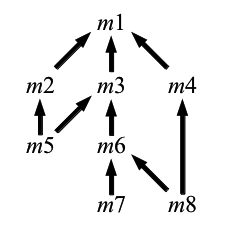
\includegraphics[width=1in,bb=0 0 228 228]{hierarchy-cropped.png}\vss}\hss}\relax
Consider a set of eight overloaded method (or function) definitions,
which for convenience we will call \emph{m1} through \emph{m8} even though
they all actually define the same name \emph{m}.  Now suppose that \emph{m2}, \emph{m3}, and \emph{m4}
are each more specific than \emph{m1};\emph{ m5} is more specific than \emph{m2} and \emph{m3};
\emph{m6} more specific than \emph{m3}; \emph{m7} more specific than \emph{m6};
and \emph{m8} more specific than \emph{m6} and \emph{m4} (see figure).
The complete ``more specific'' relation is of course the transitive closure
of the stated relationships, so that, for example,\emph{m8} is also more specific
than \emph{m1} and \emph{m3}.

The idea behind our implementation strategy is that if, for a given invocation of \emph{m},
the compiler determines that \emph{m1} is the statically most specific definition,
then at run time \emph{m1} must defer to more specific definitions.  The key insight is that,
while it is \emph{correct} for m1 to consider deferring to each of \emph{m2} through \emph{m8},
it is \emph{sufficient} for \emph{m1} to defer only to \emph{m2}, \emph{m3}, and \emph{m4}, because each of them
has the same obligation to defer.  Moreover, if \emph{m1} has more than one choice,
the choice does not matter, thanks to the Meet Rule.  For example, suppose that
at run time \emph{m8} is actually the dynamically most specific applicable definition;
then \emph{m2} must not be applicable, and \emph{m3} and \emph{m4} must be applicable.  It does not matter
whether \emph{m1} hands off responsibility to \emph{m3} or \emph{m4}; if the eventual correct choice is \emph{m8},
then repeated deferral will eventually transfer control down the lattice to \emph{m8}.

Therefore our strategy is to rewrite each function or method definition into two:
the extra function is considered the primary entry point and implements the lattice deferral strategy.
For example, \emph{m1} is augmented with a primary entry point \emph{m1entry} that has roughly this structure:
\begin{tabbing}
\emph{m1entry}: \= if \emph{m2} is applicable then call \emph{m2entry} \\
\>else if \emph{m3} is applicable then call \emph{m3entry} \\
\>else if \emph{m4} is applicable then call \emph{m4entry} \\
\>else call \emph{m1}
\end{tabbing}
Similarly, \emph{m3} is augmented with \emph{m3entry}:
\begin{tabbing}
\emph{m3entry}: \= if \emph{m5} is applicable then call \emph{m5entry} \\
\>else if \emph{m6} is applicable then call \emph{m6entry} \\
\>else call \emph{m3}
\end{tabbing}
For the sake of uniformity, \emph{m7} is augmented with \emph{m7entry}:
\begin{tabbing}
\emph{m7entry}: call \emph{m7}
\end{tabbing}
Routine inlining optimizes away such trivial entry points.

As we shall see in \secref{translation},
in practice we rewrite each definition into more than two definitions,
in order to handle the \KWD{asif} construction and some of the tricky points of
deferring dotted methods, but the basic idea of deferral down the lattice
of the ``more specific'' relation applies to both dotted methods
and top-level functions; the details differ because of the differing visibility
rules for methods and functions.
On the other hand, functional methods are handled by first rewriting them
into a collection of top-level functions and dotted methods.

The notion of being ``more specific'' comes into play only after
accessibility has been considered.  Accessibility is in turn governed
by the component system.  As a result, while there is a single dispatch
lattice for all dotted methods named \VAR{m},
there is a separate dispatch lattice for top-level functions named \VAR{f}
within each component in which some function named \VAR{f} is visible.
Importing some definitions of function \VAR{f} from component \VAR{A} to component \VAR{B}
causes corresponding entry points in component A to become part of the
dispatch lattice for \VAR{f} in component \VAR{B}.


\section{The Source Language}
\seclabel{source}

Here we summarize the source language, which is a subset of Fortress (in
particular, variables declared at the top level of a component or API are
omitted as not salient to our focus here, and declarations and uses of operator
symbols are assumed to have already been converted to declarations of ordinary
functions or functional methods and to ordinary function calls).
Please refer to \figref{source-grammar}.

A program in the source language is a collection of components and APIs; their order does not matter.

Each API contains declarations of traits and functions; their order does not matter.
(Actual Fortress APIs also allow declarations of objects and variables, but the bookkeeping
related to those is not relevant to the theme of this paper.)
An API may also import traits and functions from other APIs,
thus allowing aggregation of APIs.

Each component contains definitions of traits, objects, top-level functions, and top-level variables,
as well as (abstract) declarations of top-level functions.  A component may also import names of
traits and functions from APIs; their implementations will be supplied by other components.
A component may export one or more APIs; in order to export an API, a component must
provide a (concrete) definition corresponding to every declaration appearing in the API.
(A Fortress component can ``provide'' a definition either by containing an actual definition
or by importing it from another API; for present purposes we will require that the
component itself contain the definition.)  Importing a trait from an API enables invocation of
dotted methods declared within that trait in the API.

Import declarations can rename traits and functions as they are imported, so that the referring component
can use a name different from the one specified in the API.

A trait declaration may contain declarations and (when within a component) definitions
of dotted methods and functional methods.  A trait declaration may also contain what looks
like a declaration of a field, but (as we shall see) this is really regarded as a requirement
that appropriate getter and setter methods be defined by any implementing object.
A trait may also include any or all of three clauses that relate it to other traits and objects:
(1) A trait \VAR{A} may \VAR{extend} one or more other traits \EXP{B_{1}, B_{2}, \ldots, B_{p}}, in which case
for each \EXP{1\leq{}j\leq{}p}, \VAR{A} is a subtype of \EXP{B_{j}}, and \VAR{A} inherits all the methods of \EXP{B_{j}} that it does not override.
(2) A trait \VAR{A} may \VAR{comprise} one or more other traits \EXP{C_{1}, C_{2}, \ldots, C_{q}}, in which case
it is a static error for any trait or object \VAR{D} to extend \VAR{A} unless \VAR{D} is a subtype of (and possibly equal to) at least one \EXP{C_{j}}
for some \VAR{j} such that \EXP{1\leq{}j\leq{}q}; furthermore, each \EXP{C_{j}} must be declared in the same component as \VAR{A}
and must extend \VAR{A}.
(3) A trait \VAR{A} may \VAR{exclude} one or more other traits \EXP{E_{1}, E_{2}, \ldots, E_{r}}, in which case
it is a static error if any trait or object \VAR{F} extends \VAR{A} and also extends \EXP{E_{j}}
for any \VAR{j} such that \EXP{1\leq{}j\leq{}r}.  (The \KWD{comprises} and \KWD{excludes} clauses do not figure
prominently in this paper, but we note that they are very important in practice in a
multiple-inheritance framework in order to indicate that certain edges \emph{cannot} occur
in the type hierarchy.  Without these clauses, it would be difficult or impossible to
get certain useful method overloadings to conform to static error checks.)


\begin{figure*}[p]
\advance \baselineskip by 0.5pt  \advance\lineskiplimit by -0.5in
\begin{tabbing}
\NT{Program} \BNF\ \GROUP{ \NT{API} \ALT\ \NT{Component} }\KLEENE\ \\
\NT{API} \BNF\ \TERM{api} \NT{ApiName} \NT{Import}\KLEENE\ \GROUP{ \NT{ApiTraitDecl} \ALT\ \NT{FunctionDecl} }\KLEENE\ \TERM{end} \NT{ApiName} \\
\NT{Component} \BNF\ \TERM{component} \NT{ComponentName} \NT{Import}\KLEENE\ \NT{Export}\KLEENEPLUS\ \NT{ComponentItem}\KLEENE\ \TERM{end} \NT{ComponentName} \\
\NT{ComponentItem} \BNF\ \NT{TraitDefn} \ALT\ \NT{ObjectDefn} \ALT\ \NT{FunctionDecl} \ALT\ \NT{FunctionDefn} \ALT\ \NT{VariableDefn} \\
\NT{Import} \BNF\ \TERM{import} \NT{ApiName} \TERM{.} \TERM{\{} \NT{ImportItemList} \TERM{\}} \\
\NT{ImportItemList} \BNF\ \NT{ImportItem} \GROUP{ \TERM{,} \NT{ImportItem} }\KLEENE\ \\
\NT{ImportItem} \BNF\ \=\NT{TraitName} \GROUP{ $\mapsto$ \NT{TraitName} }\OPTIONAL\ \ALT\ \NT{FunctionName} \GROUP{ $\mapsto$ \NT{FunctionName} }\OPTIONAL\ \\
\NT{Export} \BNF\ \TERM{export} \NT{ApiName} \\
\NT{ApiTraitDecl} \BNF\ \TERM{trait} \NT{TraitName} \NT{Extends}\OPTIONAL\ \NT{Comprises}\OPTIONAL\ \NT{Excludes}\OPTIONAL\ \NT{ApiTraitItem}\KLEENE\ \TERM{end} \\
\NT{ApiTraitItem} \BNF\ \NT{VariableDecl} \ALT\ \NT{DottedMethodDecl} \ALT\ \NT{FunctionalMethodDecl} \\[6pt]
\NT{TraitDefn} \BNF\ \TERM{trait} \NT{TraitName} \NT{Extends}\OPTIONAL\ \NT{Comprises}\OPTIONAL\ \NT{Excludes}\OPTIONAL\ \NT{TraitItem}\KLEENE\ \TERM{end} \\
\NT{ObjectDefn} \BNF\ \TERM{object} \NT{ObjectName} \GROUP{ \TERM{(} \NT{ParameterList}\OPTIONAL\ \TERM{)} }\OPTIONAL\ \NT{Extends}\OPTIONAL\ \NT{ObjectItem}\KLEENE\ \TERM{end} \\
\NT{Extends} \BNF\ \TERM{extends} \TERM{\{} \NT{TraitNameList} \TERM{\}} \\
\NT{TraitNameList} \BNF\ \NT{TraitName} \GROUP{ \TERM{,} \NT{TraitName} }\KLEENE\ \\
\NT{Comprises} \BNF\ \TERM{comprises} \TERM{\{} \NT{TypeNameList} \TERM{\}} \\
\NT{Excludes} \BNF\ \TERM{excludes} \TERM{\{} \NT{TypeNameList} \TERM{\}} \\
\NT{TraitItem} \BNF\ \NT{ApiTraitItem} \ALT\ \NT{DottedMethodDefn} \ALT\ \NT{FunctionalMethodDefn} \\
\NT{ObjectItem} \BNF\ \NT{VariableDefn} \ALT\ \NT{DottedMethodDefn} \ALT\ \NT{FunctionalMethodDefn} \\[6pt]
\NT{DottedMethodDecl} \BNF\ \GROUP{ \TERM{getter} \ALT\ \TERM{setter} }\OPTIONAL\ \NT{MethodName} \TERM{(} \NT{ParameterList}\OPTIONAL\ \TERM{)} $:$ \NT{Type} \\
\NT{DottedMethodDefn} \BNF\ \NT{DottedMethodDecl} $=$ \NT{Expression} \\
\NT{FunctionalMethodDecl} \BNF\ \NT{FunctionName} \TERM{(} \NT{SelfParameterList} \TERM{)} $:$ \NT{Type} \\
\NT{FunctionalMethodDefn} \BNF\ \NT{FunctionalMethodDecl} $=$ \NT{Expression} \\
\NT{FunctionDecl} \BNF\ \NT{FunctionName} \TERM{(} \NT{ParameterList}\OPTIONAL\ \TERM{)} $:$ \NT{Type} \\
\NT{FunctionDefn} \BNF\ \NT{FunctionDecl} $=$ \NT{Expression} \\[6pt]
\NT{ParameterList} \BNF\ \NT{VariableDecl} \GROUP{ \TERM{,} \NT{VariableDecl} }\KLEENE\ \\
\NT{SelfParameterList} \BNF\ \GROUP{ \NT{VariableDecl} \TERM{,} }\KLEENE\ \TERM{self} \GROUP{ \TERM{,} \NT{VariableDecl} }\KLEENE\ \\
\NT{VariableDecl} \BNF\ \TERM{var}\OPTIONAL\ \NT{VariableName} $:$ \NT{Type} \\
\NT{VariableDefn} \BNF\ \NT{VariableDecl} \GROUP{ $=$ \ALT\ $\ASSIGN$ } \NT{Expression} \ALT\ \NT{SimpleBinding} $=$ \NT{Expression} \\
\NT{SimpleBinding} \BNF\ \NT{VariableName} \ALT\ \TERM{(} \NT{SimpleBindingList}\OPTIONAL\ \TERM{)} \\
\NT{SimpleBindingList} \BNF\ \NT{SimpleBinding} \GROUP{ \TERM{,} \NT{SimpleBinding} }\KLEENE\ \\[6pt]
\NT{Type} \BNF\ \NT{TypeName} \ALT\ \TERM{(} \NT{TypeList}\OPTIONAL\ \TERM{)} \ALT\ \NT{Type} $\rightarrow$ \NT{Type} \\
\NT{TypeList} \BNF\ \NT{Type} \GROUP{ \TERM{,} \NT{Type} }\KLEENE\ \\
\NT{TypeName} \BNF\ \NT{TraitName} \ALT\ \NT{ObjectName} \\
\NT{TypeNameList} \BNF\ \NT{TypeName} \GROUP{ \TERM{,} \NT{TypeName} }\KLEENE\ \\[6pt]
\NT{Expression} \BNF\ \=\NT{VariableName} \ALT\ \NT{Literal} \ALT\ \TERM{self} \ALT\ \TERM{(} \NT{ExpressionList}\OPTIONAL\ \TERM{)} \ALT\ \NT{Assignment}
%      \ALT\ \NT{OperatorCall}
%       \ALT\ \NT{Reduction} \ALT\ \NT{Comprehension}
    \ALT\ \\
               \>\NT{FunctionCall} \ALT\ \NT{DottedMethodCall} \ALT\ \NT{FieldAccess} \ALT\ \NT{FieldAssignment} \ALT\ \NT{IfThenElseEnd} \ALT\ \NT{DoEnd} \\
\NT{ExpressionList} ::= \NT{Expression} \GROUP{ \TERM{,} \NT{Expression} }\KLEENE\ \\
\NT{Assignment} \BNF\ \NT{VariableName} $\ASSIGN$ \NT{Expression} \\
% \NT{OperatorCall} \BNF\ \NT{Prefix} \ALT\ \NT{Postfix} \ALT\ \NT{Infix} \ALT\ \NT{Enclosing} \ALT\ \NT{Subscripted} \ALT\ \NT{SubscriptedAssignment} \\
% \NT{Prefix} \BNF\ \NT{Operator} \NT{CallExpr} \\
% \NT{PostFix} \BNF\ \NT{CallExpr} \NT{Operator} \\
% \NT{Infix} \BNF\ \NT{CallExpr} \NT{Operator} \NT{CallExpr} \\
% \NT{Operator} \BNF\ \NT{AllCapsIdentifier} \ALT\ \NT{UnicodeMathematicalOperator} \ALT\ \EXP{@} \ALT\ \EXP{\mathbin{\#}} \ALT\ \EXP{\COLONOP} \ALT\ \EXP{-} \ALT\ \EXP{!} \ALT\ \EXP{!!} \ALT\ \EXP{?} \ALT\ \EXP{\cdot} \ALT\ \EXP{/} \ALT\ 
%          \EXP{\dagger} \ALT\ \EXP{\ddag} \ALT\ \EXP{\bullet} \ALT\ \ldots\  and a few others \\
% \NT{UnicodeMathematicalOperator} \BNF\ \EXP{+} \ALT\ \EXP{\times} \ALT\ \EXP{\div} \ALT\ \EXP{=} \ALT\ \EXP{\neq} \ALT\ \EXP{<} \ALT\ \EXP{\leq} \ALT\ \EXP{\geq} \ALT\ \EXP{>} \ALT\ \EXP{\nless} \ALT\ \EXP{\nleq} \ALT\ \EXP{\ngeq} \ALT\ \EXP{\ngtr} \ALT\ 
%         \EXP{\equiv} \ALT\ \EXP{\not\equiv} \ALT\ \EXP{\sequiv} \ALT\ \EXP{\not\sequiv} \ALT\ \EXP{\approx} \ALT\ \EXP{\not\approx} \ALT\ \EXP{\simeq} \ALT\ \EXP{\not\simeq} \ALT\ \\
% \qquad  \EXP{\cup} \ALT\ \EXP{\cap} \ALT\ \EXP{\subset} \ALT\ \EXP{\subseteq} \ALT\ \EXP{\supseteq} \ALT\ \EXP{\supset} \ALT\ \EXP{\not\subset} \ALT\ \EXP{\nsubseteq} \ALT\ \EXP{\nsupseteq} \ALT\ \EXP{\not\supset} \ALT\
%         \EXP{\oplus} \ALT\ \EXP{\ominus} \ALT\ \EXP{\otimes} \ALT\ \EXP{\oslash} \ALT\ \EXP{\odot} \ALT\  \EXP{\in} \ALT\ \EXP{\ni} \ALT\ \EXP{\notin} \ALT\ \EXP{\not\ni} \ALT\ 
%         \EXP{\Subset} \ALT\ \EXP{\Supset} \ALT\ \EXP{\Cap} \ALT\ \EXP{\Cup} \ALT\ \EXP{\uplus} \ALT\ \EXP{\precsim} \ALT\ \EXP{\succsim} \ALT\ \EXP{\sum} \ALT\ \EXP{\prod} \ALT\ \\
% \qquad  \EXP{\sqcup} \ALT\ \EXP{\sqcap} \ALT\ \EXP{\sqsubset} \ALT\ \EXP{\sqsubseteq} \ALT\ \EXP{\sqsupseteq} \ALT\ \EXP{\sqsupset} \ALT\ \EXP{\not\sqsubset} \ALT\ \EXP{\not\sqsubseteq} \ALT\ \EXP{\not\sqsupseteq} \ALT\ \EXP{\not\sqsupset} \ALT\
%         \EXP{\boxplus} \ALT\ \EXP{\boxminus} \ALT\ \EXP{\boxtimes} \ALT\ \EXP{\boxslash} \ALT\ \EXP{\boxdot} \ALT\ 
%         \EXP{\Join} \ALT\ \EXP{\ltimes} \ALT\ \EXP{\rtimes} \ALT\ 
%         \EXP{\vdash} \ALT\ \EXP{\dashv} \ALT\ \EXP{\partial} \ALT\ \EXP{\sim} \ALT\ \EXP{\leftrightarrows} \ALT\ \EXP{\setminus} \ALT\ \EXP{\mapsto} \ALT\ \EXP{\bumpeq} \ALT\ \EXP{\Bumpeq} \ALT\ \EXP{\circeq} \ALT\ \\
% \setbox0\hbox{$\sqcap$}\relax
% \qquad  \EXP{\hbox to \wd0{\hss$\curlywedge$\hss}} \ALT\ \EXP{\hbox to \wd0{\hss$\curlyvee$\hss}} \ALT\ \EXP{\prec} \ALT\ \EXP{\preccurlyeq} \ALT\ \EXP{\succcurlyeq} \ALT\ \EXP{\succ} \ALT\ \EXP{\nprec} \ALT\ \EXP{\not\preccurlyeq} \ALT\ \EXP{\not\succcurlyeq} \ALT\ \EXP{\nsucc} \ALT\
%         \EXP{\dotplus} \ALT\ \EXP{\dotminus} \ALT\ \EXP{\dottimes} \ALT\ \EXP{\pm} \ALT\ \EXP{\mp} \ALT\
%         \EXP{\lhd} \ALT\ \EXP{\unlhd} \ALT\ \EXP{\rhd} \ALT\ \EXP{\unrhd} \ALT\ 
%         \EXP{\ntriangleleft} \ALT\ \EXP{\ntriangleright} \ALT\ \EXP{\ntrianglelefteq} \ALT\ \EXP{\ntrianglerighteq}
%         \ALT\ \EXP{\circledcirc} \ALT\ \EXP{\diamond} \ALT\ \EXP{\surd} \ALT\ \EXP{\propto} \ALT\ \EXP{\star} \ALT\ \\
% \qquad  \EXP{\wedge} \ALT\ \EXP{\vee} \ALT\ \EXP{\nand} \ALT\ \EXP{\nor} \ALT\ \EXP{\xor} \ALT\ \EXP{\rightarrow} \ALT\ \EXP{\leftrightarrow} \ALT\ \EXP{\leftarrow} \ALT\ \EXP{\neg} \ALT\ \EXP{\lessdot} \ALT\ \EXP{\gtrdot} \ALT\ 
%         \EXP{\uparrow} \ALT\ \EXP{\downarrow} \ALT\ \EXP{\updownarrow} \ALT\ \EXP{\Rightarrow} \ALT\ \EXP{\Leftrightarrow} \ALT\ \EXP{\Leftarrow} \ALT\ \EXP{\Uparrow} \ALT\ \EXP{\Downarrow} \ALT\ \EXP{\Updownarrow} \ALT\ 
%         \EXP{\mid} \ALT\ \EXP{\mathrel{\Vert}} \ALT\ \EXP{\circ} \ALT\ \ldots\  and many others  \\
% \NT{Enclosing} \BNF\ \=\EXP{[} \NT{CallExprList}\OPTIONAL\ \EXP{]} \ALT\ 
%         \EXP{\lfloor} \NT{CallExprList}\OPTIONAL\ \EXP{\rfloor} \ALT\ \EXP{\lceil} \NT{CallExprList}\OPTIONAL\ \EXP{\rceil} \ALT\
%         \EXP{\lhfloor} \NT{CallExprList}\OPTIONAL\ \EXP{\rhfloor} \ALT\ \EXP{\lhceil} \NT{CallExprList}\OPTIONAL\ \EXP{\rhceil} \ALT\ \\
% \>      \EXP{\lbrace} \NT{CallExprList}\OPTIONAL\ \EXP{\rbrace} \ALT\ 
%         \EXP{\langle} \NT{CallExprList}\OPTIONAL\ \EXP{\rangle} \ALT\ \EXP{\langle\mskip-5mu\langle} \NT{CallExprList}\OPTIONAL\ \EXP{\rangle\mskip-5mu\rangle} \ALT\ 
%         \EXP{\ulcorner} \NT{CallExprList}\OPTIONAL\ \EXP{\urcorner} \ALT\  \EXP{\llcorner} \NT{CallExprList}\OPTIONAL\ \EXP{\lrcorner} \ALT\ \\
% \>      \EXP{\{\mskip-4mu|} \NT{CallExprList}\OPTIONAL\ \EXP{|\mskip-4mu\}} \ALT\ \EXP{\langle\mskip-4mu\cdot} \NT{CallExprList}\OPTIONAL\ \EXP{\cdot\mskip-4mu\rangle} \ALT\  
%         \EXP{\langle\mskip-3.7mu|} \NT{CallExprList}\OPTIONAL\ \EXP{|\mskip-3.7mu\rangle} \ALT\ \EXP{\mathrel{\Vert}} \NT{CallExprList}\OPTIONAL\ \EXP{\mathrel{\Vert}} \ALT\
%          \ldots\  and many others \\
% \NT{Subscripted} \BNF\ \NT{CallExpr} \NT{Enclosing} \\
% \NT{SubscriptedAssignment} \BNF\ \NT{Subscripted} $\ASSIGN$ \NT{CallExpr} \\
\NT{FunctionCall} \BNF\ \NT{FunctionName} \TERM{(} \NT{CallExprList}\OPTIONAL\ \TERM{)} \\
\NT{DottedMethodCall} \BNF\ \NT{CallExpr} \TERM{.} \NT{MethodName} \TERM{(} \NT{CallExprList}\OPTIONAL\ \TERM{)} \\
\NT{CallExpr} \BNF\ \NT{Expression} \GROUP{ \TERM{asif} \NT{Type} }\OPTIONAL\ \\
\NT{CallExprList} \BNF\ \NT{CallExpr} \GROUP{ \TERM{,} \NT{CallExpr} }\KLEENE\ \\
\NT{FieldAccess} \BNF\ \NT{CallExpr} \TERM{.} \NT{VariableName} \\
\NT{FieldAssignment} \BNF\ \NT{CallExpr} \TERM{.} \NT{VariableName} $\ASSIGN$ \NT{CallExpr} \\
\NT{IfThenElseEnd} \BNF\ \=\TERM{if} \NT{Expression} \TERM{then} \NT{StatementList} \GROUP{ \TERM{elif} \NT{Expression} \TERM{then} \NT{StatementList} }\KLEENE\ \GROUP{ \TERM{else} \NT{StatementList} }\OPTIONAL\ \TERM{end} \\
\NT{DoEnd} \BNF\ \TERM{do} \NT{StatementList} \TERM{end} \\
\NT{StatementList} \BNF\ \GROUP{ \NT{FunctionDefn} \ALT\ \NT{VariableDefn} \ALT\ \NT{Expression} }\KLEENE\ \NT{Expression}
\end{tabbing}
\vskip-8pt
\caption{Grammar for source language}
\figlabel{source-grammar}
\end{figure*}


\begin{figure*}[t]
\advance \baselineskip by 0.5pt  \advance\lineskiplimit by -0.5in
\begin{tabbing}
\NT{Program} \BNF\ \GROUP{ \NT{FunctionDefn} \ALT\ \NT{InterfaceDefn} \ALT\ \NT{ClassDefn} \ALT\ \NT{VariableDefn} }\KLEENE\ \\
\NT{InterfaceDefn} \BNF\ \TERM{interface} \NT{InterfaceName} \NT{Extends}\OPTIONAL\ \NT{DottedMethodDecl}\KLEENE\ \TERM{end} \\
\NT{ClassDefn} \BNF\ \TERM{class} \NT{ClassName} \NT{Extends}\OPTIONAL\ \NT{Constructor} \NT{ClassItem}\KLEENE\ \TERM{end} \\
\NT{Extends} \BNF\ \TERM{extends} \TERM{\{} \NT{InterfaceNameList} \TERM{\}} \\
\NT{InterfaceNameList} \BNF\ \NT{InterfaceName} \GROUP{ \TERM{,} \NT{InterfaceName} }\KLEENE\ \\
\NT{Constructor} \BNF\ \TERM{constructor} \NT{ClassName} \TERM{(} \NT{ParameterList}\OPTIONAL\ \TERM{)} $=$ \NT{Expression} \\
\NT{ClassItem} \BNF\ \NT{VariableDefn} \ALT\ \NT{DottedMethodDefn} \\[6pt]
\NT{DottedMethodDecl} \BNF\ \NT{MethodName} \TERM{(} \NT{ParameterList}\OPTIONAL\ \TERM{)} $:$ \NT{Type} \\
\NT{DottedMethodDefn} \BNF\ \NT{DottedMethodDecl} $=$ \NT{Expression} \\
\NT{FunctionDefn} \BNF\ \NT{FunctionName} \TERM{(} \NT{ParameterList}\OPTIONAL\ \TERM{)} $:$ \NT{Type} $=$ \NT{Expression} \\[6pt]
\NT{ParameterList} \BNF\ \NT{VariableDecl} \GROUP{ \TERM{,} \NT{VariableDecl} }\KLEENE\ \\
\NT{VariableDecl} \BNF\ \TERM{var}\OPTIONAL\ \NT{VariableName} $:$ \NT{Type} \\
\NT{VariableDefn} \BNF\ \NT{VariableDecl} \GROUP{ $=$ \ALT\ $\ASSIGN$ } \NT{Expression} \ALT\ \NT{SimpleBinding} $=$ \NT{Expression} \\
\NT{SimpleBinding} \BNF\ \NT{VariableName} \ALT\ \TERM{(} \NT{SimpleBindingList}\OPTIONAL\ \TERM{)} \\
\NT{SimpleBindingList} \BNF\ \NT{SimpleBinding} \GROUP{ \TERM{,} \NT{SimpleBinding} }\KLEENE\ \\[6pt]
\NT{Type} \BNF\ \NT{TypeName} \ALT\ \TERM{(} \NT{TypeList}\OPTIONAL\ \TERM{)} \ALT\ \NT{Type} $\rightarrow$ \NT{Type} \\
\NT{TypeList} \BNF\ \NT{Type} \GROUP{ \TERM{,} \NT{Type} }\KLEENE\ \\
\NT{TypeName} \BNF\ \NT{InterfaceName} \ALT\ \NT{ClassName} \\[6pt]
\NT{Expression} \BNF\ \=\NT{VariableName} \ALT\ \NT{Literal} \ALT\ \TERM{self} \ALT\ \TERM{(} \NT{ExpressionList}\OPTIONAL\ \TERM{)} \ALT\ \NT{Assignment} \ALT\ \\
               \>\NT{TypeLiteral} \ALT\ \NT{TypeTest} \ALT\ \NT{Construction} \ALT\ \NT{Conjunction} \ALT\ \\
               \>\NT{FunctionCall} \ALT\ \NT{DottedMethodCall} \ALT\ \NT{FieldAccess} \ALT\ \NT{FieldAssignment} \ALT\ \NT{IfThenElseEnd} \ALT\ \NT{DoEnd} \\
\NT{ExpressionList} ::= \NT{Expression} \GROUP{ \TERM{,} \NT{Expression} }\KLEENE\ \\
\NT{TypeLiteral} \BNF\ \NT{Type} \TERM{.} \TERM{type} \\
\NT{TypeTest} \BNF\ \NT{Expression} \TERM{instanceof} \NT{Type} \\
\NT{Construction} \BNF\ \TERM{new} \NT{ClassName} \TERM{(} \NT{ExpressionList}\OPTIONAL\ \TERM{)} \\
\NT{Assignment} \BNF\ \NT{VariableName} $\ASSIGN$ \NT{Expression} \\
\NT{Conjunction} \BNF\ \NT{Expression} {\tt \char'46\char'46} \NT{Expression} \\
\NT{FunctionCall} \BNF\ \NT{FunctionName} \TERM{(} \NT{ExpressionList}\OPTIONAL\ \TERM{)} \\
\NT{DottedMethodCall} \BNF\ \NT{Expression} \TERM{.} \NT{MethodName} \TERM{(} \NT{ExpressionList}\OPTIONAL\ \TERM{)} \\
\NT{FieldAccess} \BNF\ \TERM{self} \TERM{.} \NT{VariableName} \\
\NT{FieldAssignment} \BNF\ \TERM{self} \TERM{.} \NT{VariableName} $\ASSIGN$ \NT{Expression} \\
\NT{IfThenElseEnd} \BNF\ \=\TERM{if} \NT{Expression} \TERM{then} \NT{StatementList} \GROUP{ \TERM{elif} \NT{Expression} \TERM{then} \NT{StatementList} }\KLEENE\ \GROUP{ \TERM{else} \NT{StatementList} }\OPTIONAL\ \TERM{end} \\
\NT{DoEnd} \BNF\ \TERM{do} \NT{StatementList} \TERM{end} \\
\NT{StatementList} \BNF\ \GROUP{ \NT{FunctionDefn} \ALT\ \NT{VariableDefn} \ALT\ \NT{Expression} }\KLEENE\ \NT{Expression}
\end{tabbing}
\vskip-8pt
\caption{Grammar for target language}
\figlabel{target-grammar}
\end{figure*}


Object declarations may contain definitions of dotted methods, functional methods, and variables;
variable definitions within an object declaration are regarded as fields of the object.
An object declaration may contain an \KWD{extends} clause that mentions supertraits,
just as for a trait declaration; in effect, an \KWD{object} declaration declares a trait of
the same name that serves as a type name, but there is no need for such a trait
to have a \KWD{comprises} clause or \KWD{excludes} clause because it cannot have subtraits.
Each object type implicitly excludes every other object type,
and indeed every type that is not its ancestor in the trait hierarchy.

If an object declaration has a parameter list, then there is an implicit top-level constructor
function with the same name, and each invocation of the constructor function returns
a fresh object whose ilk is the implicit trait of that same name; moreover, each parameter
is also a field of the freshly constructed object.
This constructor function can participate in an overload set with ordinary functions and
functional methods of the same name.
If an object declaration has no
parameter list, then it represents a \emph{singleton object} whose ilk is the implicit trait
with the same name, and there is an implicit top-level variable with the same name whose value
is that singleton object.

A dotted method declaration or definition is much as in the Java language, with slightly different syntax.
A dotted method with the \KWD{getter} keyword is invoked by a field access,
and a dotted method with the \KWD{setter} keyword is invoked by a field assignment.
Such a getter or setter method must not be present in the same trait or
object declaration as a field declaration or definition with the same name.
Functional method declarations are distinguished syntactically from dotted method
declarations by the presence of the keyword \EXP{\KWDVAR{self}} in (exactly one place in) the parameter list.

Variable declarations specify a name and a type; if the keyword \KWD{var} is present,
the variable is mutable.  Variable definitions additionally
specify an expression that provides an initial value.  The symbol \EXP{=} indicates
definition of an immutable variable; the symbol \EXP{\ASSIGN} (which is also used for assignment) indicates
definition of a mutable variable (in which case \KWD{var} may optionally appear).
As a convenience, within a statement list, a tuple of simple variable names may be bound to the
respective elements of a tuple value.

A type may be the declared name of a trait or object, a parenthesized type, a
tuple of types, or an arrow type.  (The interesting issue of what is the
precise type of an overloaded function name when used as a value
is beyond the scope of this paper.)

Names of types are in a different namespace from the names
of variables and functions; one may have a type and a function, or a type and a variable,
with the same name.
Definitions and declarations of local function and variables are not permitted to shadow
outer definitions or declarations with the same name.

The Fortress parser rewrites operator syntax into function calls in a conventional manner,
so there is no need to model operators separately in our source language here.

A function call may invoke either an ordinary function, a functional method, or an object constructor---but
if the function call occurs within a trait
or object declaration that has or inherits a definition or declaration
of a dotted method with the same name, then it is considered to
invoke that dotted method with \EXP{\KWDVAR{self}} as the receiver.
(This ``convenience abbreviation'' of a dotted method call---allowing the elision
of a leading ``\EXP{\KWDVAR{self}.\!}'' or ``\EXP{\KWDVAR{this}.\!}''---will
be familiar to programmers who use the Java language~\cite[\S 15.11]{JLS1}.)

Within an invocation of a dotted method or functional method,
% , or operator functional method,
an immediate subexpression (that is, an argument expression or receiver expression)
may have the form \EXP{x \KWD{asif} T} where \VAR{x} is an expression and \VAR{T} is a type;
this is used to get the effect of the Java {\tt super} construct, but specifies
that \VAR{T} is the specific supertype of interest.  If any subexpression of an invocation
is an \KWD{asif} expression, then the subexpression before the dot (in a dotted method call)
or corresponding to the \EXP{\KWDVAR{self}} parameter of the statically most specific applicable declaration
or definition, which must be a declaration or definition of a functional method (in a function call),
must also be an \KWD{asif} expression.

Within a block (which for present purposes we may regard as identical to
a \NT{StatementList}, though the actual Fortress grammar draws a subtle distinction
for the purpose of defining mutually recursive functions),
functions and variables may be defined locally.

% Fortress expression syntax includes comprehensions such as \EXP{\lbrace\,x \mid x \leftarrow\; \KWDVAR{self}, x \in \VAR{other}\,\rbrace}
% and reductions such as \EXP{\prod\limits_{k\leftarrow1\COLONOP{}n}\, k}.
% They appear in this paper only as brief examples.

% Any all-caps identifier (of more than one letter) or Unicode mathematical operator may be used as an
% operator.  Any operator may be overloaded not only with respect to parameter types but also
% with respect to whether it is prefix, postfix, or infix.  (For the purposes of this paper,
% we gloss over the details of how the Fortress parser resolves fixity and precedence.)

Identifiers may include any Unicode letter, digit or connecting punctuation, but not dollar signs ``\$'.



\section{The Target Language}
\seclabel{target}

Here we summarize the features of the target language that differ from those of the source language.  Please refer to \figref{target-grammar}.

A target-language program consists of a set of definitions of interfaces, classes, top-level functions,
and top-level variables.  There are no components or APIs.  A target-language program
is much like a single Java compilation unit.

Interface declarations contain only dotted method declarations;
there is no executable code in an interface.
There are no functional methods.
Methods cannot be overloaded, and \KWD{comprises} and \KWD{excludes} clauses are unnecessary.

Class declarations are similar to those in the Java language.
Every class declaration has a {\tt constructor} declaration;
a constructor is invoked by a construction expression beginning with the keyword {\tt new}.
Class declarations may contain dotted method definitions,
as well as declarations and definitions of fields.

For convenience, the target language includes the short-circuit (that is, conditional)
Boolean {\sc and} operator {\tt \char'46\char'46}, as well as the {\tt instanceof} operator
that can test whether the value of an expression belongs to a specified type.
If a variable passes an {\tt instanceof} check in the predicate part of
an \KWD{if} statement, then the variable is regarded as having that type in the corresponding
\KWD{then} branch of the \KWD{if} statement (thus no cast is required).

An expression of the form \EXP{T.\!\KWD{type}} is a \emph{type literal}
(analogous to an expression of the form \EXP{T.\!\KWD{class}} in the Java language);
its value (which is of type \TYP{Type}) is a run-time reification of the type \VAR{T}.  Such an object
provides a dotted method \EXP{t.\VAR{isSubtype}(u)} where \VAR{u} is also such an object,
which returns \VAR{true} if the type represented by \VAR{t} is a subtype of
(possibly the same as) the type represented by \VAR{u}, and otherwise
returns \VAR{false}.  (Compare the method {\tt isAssignableFrom} of the Java class {\tt class},
which provides the converse ``is a supertype'' test.)

Every value $x$ provides the dotted method \EXP{x.\VAR{ilk}(\ultrathin)}, which returns
a reified type object that represents the ilk of the object, function, or tuple.
The reified ilk of a function is of type \TYP{ArrowType},
and provides additional methods such as \VAR{argumentType} and \VAR{resultType},
which for a function type \EXP{D\rightarrow{}R} return reified type objects for \VAR{D} and \VAR{R}, respectively.
(Reified tuple types also have extra methods, but
we will not need them for our exposition here.)

Field accesses and assignments are supported, but only within class declarations,
and the expression before the dot must be \EXP{\KWDVAR{self}}.

It is convenient to assume that target-language 
identifiers, in addition to Unicode letters, digits, and connecting punctuation,
may also include a character ``\$' that cannot appear in source-language identifiers,
in order to allow construction of ``mangled'' names that cannot conflict with
identifiers originating in source-language code.
%(In effect, mangled names are little record structures to be processed by the linker.)
In what follows, it is assumed
that any target-language identifier containing one or more ``\$' characters
and also one or more variables mentioned in the text actually represents
an identifier constructed by substituting some string value (a name or
the decimal representation of an integer value) for each variable.
For example, if we say that \EXP{j=3} and \VAR{w} stands for the name \VAR{foo},
then \VAR{w\$j\$dispatch} stands for the identifier \VAR{foo\$\mathrm{3}\$dispatch}.




\section{Details of the Translation}
\seclabel{translation}

The purpose of this section is to explain some of the detailed semantics
of the source language outlined in \secref{source} by showing
how to translate it into the much simpler target language outlined
in \secref{target}.

To summarize, the source language has these features of interest:
\begin{trivlist}\leftskip=1em \itemindent=-\leftskip
\item[] a static type system;
\item[] traits and objects can extend multiple traits;
\item[] multiple inheritance of both dotted and functional methods;
\item[] both objects and traits can contain both declarations and definitions of both dotted and functional methods;
\item[] fields are declared only in objects;
\item[] objects cannot extend other objects;
\item[] dotted methods, functional methods, top-level functions, and local functions all support symmetric dynamic multimethod dispatch among overloaded definitions;
\item[] an ``{\tt asif}'' feature to get ``{\tt super}''-like behavior in a multiple-inheritance, symmetric-dispatch environment;
\item[] a rule that overloaded definitions must form a meet-bounded lattice, thereby making it impossible for any function or method call to be ambiguous;
\item[] a system of modular components and APIs that allows controlled import and export of names of individual traits, objects, top-level functions, and top-level variables; and
\item[] separate compilation, and therefore separate static type-checking, of components.
\end{trivlist}
and the target language has these features and limitations:
\begin{trivlist}\leftskip=1em \itemindent=-\leftskip
\item[] a static type system;
\item[] interfaces and classes can extend multiple interfaces;
\item[] multiple inheritance of dotted methods
\item[] interfaces can contain only abstract dotted method declarations;
\item[] classes can contain concrete dotted method declarations;
\item[] fields are declared only in classes;
\item[] classes do not extend other classes;
\item[] no overloading or overriding, and no inheritance of concrete method definitions;
\item[] no ``{\tt super}'' feature of any kind;
\item[] field access occurs only within the dotted methods of the declaring class;
\item[] dotted methods need dispatch only on the receiver;
\item[] top-level functions and local functions are not overloaded and therefore require no dispatch;
\item[] one global namespace and no separate compilation;
\item[] the minimal reflective ability to obtain a ``type object'' representing either
an arbitrary type or the ilk (run-time type) of an object, and to inquire of
two such type objects whether one represents a subtype of the other.
\end{trivlist}

The rewriting does not group a set of overloaded methods or functions into a monolithic ``generic'' method or function;
rather, the implementation of the dispatch process is distributed in a manner that allows selective export and selective optimization.
The source language captures essential features of the multimethod dispatch mechanism of the Fortress programming language.
The target language is considerably simpler than the Java programming language and is readily supported by the Java Virtual Machine.
The demonstrated rewriting is a practical basis for separate compilation and is easily extended to the case of
explicitly type-polymorphic methods and functions.

The big picture: trait declarations are rewritten into interface declarations,
object definitions are rewritten into class definitions,
fields are largely eliminated by using getter and setter methods,
and functional method definitions are eliminated by translating them into
top-level function definitions that serve as trampolines to corresponding
dotted method definitions.  Namespaces are eliminated by mangling names
to include the name of the defining component.

The source program is first subjected to static analysis,
including verification of syntactic well-formedness, static type checking,
and verification that every overload set obeys the Meet Rule.
Intermediate stages of the rewriting process do not
maintain either well-formedness or type correctness according to either
source-language or target-language rules, but the final result
should be well-formed and type-correct according to target-language rules,
and its execution behavior is intended to be identical to (and thereby \emph{explain})
the execution behavior of the original source-language program.

We describe a series of rewriting steps as if each step were applied
to all components and APIs before proceeding to the next step.
However, up until the last step, ``linking and final assembly''
(see \secref{linking}),
each component may be processed entirely independently of all other
components, relying only on information imported from APIs.


% \subsection{Eliminate Operator Syntax}

% Syntactic sugar associated with the definition
% and use of operator characters (and this includes array access and assignment)
% is rewritten into definitions and uses of functions or functional methods.
% This transformation phase is conceptually straightforward,
% so we present representative examples here rather than explaining
% numerous special cases exhaustively.

% \begin{figure*}[t]
% \divide\tabcolsep by 2
% \begin{tabular}{@{}lll@{}}
% \hbox to 2.547in{\EXP{\KWD{opr}\, \mathord{+}(p\COLON \TYP{Number}, q\COLON \TYP{Number})\COLON \TYP{Number}}} & becomes &
%   \EXP{\VAR{infix\$\hbox{\rm\sc plus}}(p\COLON \TYP{Number}, q\COLON \TYP{Number})\COLON \TYP{Number}} \\
% \EXP{\KWD{opr} (n\COLON \mathbb{N})\mathord{!}\: \COLONOP \mathbb{N} = \prod\limits_{k\leftarrow1\COLONOP{}n}\, k} & becomes &
%   \EXP{\VAR{postfix\$\hbox{\rm\sc exclamation{\tt\_\verythin}mark}}(n\COLON \mathbb{N})\COLON \mathbb{N} = \prod\limits_{k\leftarrow1\COLONOP{}n}\, k} \\
% \EXP{\KWD{opr}\, {\textstyle\sqrt{x\COLON \mathbb{R}64}}\COLON \mathbb{R}64 = x.\VAR{sqrt}(\ultrathin)} & becomes &
%   \EXP{\VAR{prefix\$\hbox{\rm\sc sqrt}}(x\COLON \mathbb{R}64)\COLON \mathbb{R}64 = x.\VAR{sqrt}(\ultrathin)} \\
% \EXP{\KWD{opr}\, \mathord{\OPR{MAX}}(\KWDVAR{self}, \VAR{other}\COLON \mathbb{Q})\COLON \mathbb{Q} =} & becomes &
%   \EXP{\VAR{infix\$\hbox{\rm\sc max}}(\KWDVAR{self}, \VAR{other}\COLON \mathbb{Q})\COLON \mathbb{Q} =} \\
% \(\2\)\EXP{\KWD{if} \VAR{other} > \KWDVAR{self} \KWD{then} \VAR{other} \KWD{else} \KWDVAR{self} \KWD{end}} & &
%   \EXP{\2\KWD{if} \VAR{other} > \KWDVAR{self} \KWD{then} \VAR{other} \KWD{else} \KWDVAR{self} \KWD{end}} \\
% \EXP{\KWD{opr}\, \mathord{\cap}(\KWDVAR{self}, \VAR{other}\COLON \TYP{Set})\COLON \TYP{Set} =} & becomes &
%   \EXP{\VAR{infix\$\hbox{\rm\sc intersection}}(\KWDVAR{self}, \VAR{other}\COLON \TYP{Set})\COLON \TYP{Set} =} \\
% \(\2\)\EXP{\lbrace\,x \mid x \leftarrow\; \KWDVAR{self}, x \in \VAR{other}\,\rbrace} & &
%   \EXP{\2\lbrace\,x \mid x \leftarrow\; \KWDVAR{self}, x \in \VAR{other}\,\rbrace} \\
% \EXP{\KWD{opr}\, \mathopen{\vert}\KWDVAR{self}\mathclose{\vert} \COLON \mathbb{N} = \KWDVAR{self}.\VAR{length}} & becomes &
%   \EXP{\VAR{enclosing\$\hbox{\rm\sc vertical{\tt\_\verythin}bar}\$\hbox{\rm\sc vertical{\tt\_\verythin}bar}}(\KWDVAR{self})\COLON \mathbb{N} = \KWDVAR{self}.\VAR{length}} \\
% \EXP{\KWD{opr}\, \lfloor{}x\COLON \mathbb{Q}\rfloor \COLONOP \mathbb{Z} = x.\VAR{floor}(\ultrathin)} & becomes &
%   \EXP{\VAR{enclosing\$\hbox{\rm\sc left{\tt\_\verythin}floor}\$\hbox{\rm\sc right{\tt\_\verythin}floor}}(x\COLON \mathbb{Q})\COLON \mathbb{Z} = x.\VAR{floor}(\ultrathin)} \\
% \EXP{\KWD{opr}\, [i\COLON \mathbb{Z}32, j\COLON \mathbb{Z}32]} & becomes &
%   \EXP{\VAR{subscript\$\hbox{\rm\sc left{\tt\_\verythin}bracket}\$\hbox{\rm\sc right{\tt\_\verythin}bracket}}(\KWDVAR{self}, i\COLON \mathbb{Z}32, j\COLON \mathbb{Z}32)} \\
% \EXP{\KWD{opr}\, [k\COLON \mathbb{N}] \ASSIGN (\VAR{newVal}\COLON \TYP{EltType})} & becomes &
%   \EXP{\VAR{assign\$\hbox{\rm\sc left{\tt\_\verythin}bracket}\$\hbox{\rm\sc right{\tt\_\verythin}bracket}}(\KWDVAR{self}, k\COLON \mathbb{N}, \VAR{newVal}\COLON \TYP{EltType})}
% \end{tabular}
% \caption{Example rewritings of declarations and definitions for operator functions and functional methods}
% \figlabel{opr-defs}
% \end{figure*}


% \begin{figure*}[t]
% \divide\tabcolsep by 2
% \begin{tabular}{@{\hskip 1.447in}lll@{}}
% \hbox to 1.1in{\EXP{a+b}} & becomes &
%   \EXP{\VAR{infix\$\hbox{\rm\sc plus}}(a, b)} \\
% \EXP{(m+1)!} & becomes &
%   \EXP{\VAR{postfix\$\hbox{\rm\sc exclamation{\tt\_\verythin}mark}}(\VAR{infix\$\hbox{\rm\sc plus}}(m, 1))} \\
% \EXP{\sqrt{ z}} & becomes &
%   \EXP{\VAR{prefix\$\hbox{\rm\sc sqrt}}(z)} \\
% \EXP{a \OPR{MAX} b} & becomes &
%   \EXP{\VAR{infix\$\hbox{\rm\sc max}}(a, b)} \\
% \EXP{C \cap D} & becomes &
%   \EXP{\VAR{infix\$\hbox{\rm\sc intersection}}(C, D)} \\
% \EXP{ \mathopen{\vert}\VAR{myArray}\mathclose{\vert} } & becomes &
%   \EXP{\VAR{enclosing\$\hbox{\rm\sc vertical{\tt\_\verythin}bar}\$\hbox{\rm\sc vertical{\tt\_\verythin}bar}}(\VAR{myArray})} \\
% \EXP{\left\lfloor{\textstyle{}n\over\textstyle2}\right\rfloor} & becomes &
%   \EXP{\VAR{enclosing\$\hbox{\rm\sc left{\tt\_\verythin}floor}\$\hbox{\rm\sc right{\tt\_\verythin}floor}}(\VAR{infix\$\hbox{\rm\sc solidus}}(n, 2))} \\
% \EXP{\VAR{myMatrix}[3, m]} & becomes &
%   \EXP{\VAR{subscript\$\hbox{\rm\sc left{\tt\_\verythin}bracket}\$\hbox{\rm\sc right{\tt\_\verythin}bracket}}(\VAR{myMatrix}, 3, m)} \\
% \EXP{\VAR{myArray}[n] \ASSIGN 17} & becomes &
%   \EXP{\VAR{assign\$\hbox{\rm\sc left{\tt\_\verythin}bracket}\$\hbox{\rm\sc right{\tt\_\verythin}bracket}}(\VAR{myArray}, n, 17)}
% \end{tabular}
% \caption{Example rewritings of uses of operators}
% \figlabel{opr-uses}
% \end{figure*}

% Each operator declaration or definition is rewritten
% into a declaration or definition of an ordinary function or functional method with a name that is based on the
% operator's syntax (infix, prefix, postfix, or enclosing) and its name
% or Unicode character name(s) (see \figref{opr-defs}).
% Similarly, operator uses are rewritten into ordinary function calls (see \figref{opr-uses}).
% (For very common characters, shortened forms of Unicode names are used.
% In the figures, note that \EXP{\mathbb{Z}} is the type of all integers (analogous to class {\tt BigInteger} in the Java language),
% \EXP{\mathbb{N}} is the type of all nonnegative integers, \EXP{\mathbb{Q}} is the type of all rational numbers,
% and \EXP{\mathbb{R}64} is the type of 64-bit IEEE 754
% floating-point numbers excluding infinities and NaN.)

% Comprehensions and reductions are also rewritten in terms of calls to higher-order methods and functions
% that take functions as arguments; the details are beyond the scope of this paper.


\subsection{Create Object Constructors}

If an object declaration with name \EXP{\mathrm{U}} has a \NT{ParameterList}
\begin{codeexamplesize}
\begin{tabbing}
\EXP{(p_{1}\COLON \mathrm{T}_{1}, p_{2}\COLON \mathrm{T}_{2}, \ldots, p_{n}\COLON \mathrm{T}_{n})}   
\end{tabbing}
\end{codeexamplesize}
then copy each variable declaration \EXP{p_{j}\COLON \mathrm{T}_{j}} from the parameter list into the
object declaration itself, adding the \KWD{var} keyword
to each one that does not already have a \KWD{var} keyword.
Then add to the object declaration a constructor definition of the form:
\begin{codeexamplesize}
\begin{tabbing}
\EXP{\KWD{constructor} \TYP{U}(p_{1}\COLON \mathrm{T}_{1}, p_{2}\COLON \mathrm{T}_{2}, \ldots, p_{n}\COLON \mathrm{T}_{n}) =\; \KWD{do}} \\
\(\2\)\EXP{\KWDVAR{self}.\VAR{field\$p}_{1} \ASSIGN p_{1}} \\
\(\2\)\EXP{\KWDVAR{self}.\VAR{field\$p}_{2} \ASSIGN p_{2}} \\
\(\2\)\EXP{\ldots} \\
\(\2\)\EXP{\KWDVAR{self}.\VAR{field\$p}_{n} \ASSIGN p_{n}} \\
\EXP{\KWD{end}}
\end{tabbing}
\end{codeexamplesize}
and delete the \NT{ParameterList} and its surrounding parentheses
from the object declaration.  If the object declaration appears in a component,
then add this top-level function definition to the component:
\begin{codeexamplesize}
\begin{tabbing}
\EXP{\TYP{U}(p_{1}\COLON \mathrm{T}_{1}, p_{2}\COLON \mathrm{T}_{2}, \ldots, p_{n}\COLON \mathrm{T}_{n})\COLON \TYP{U} =\;\KWD{new} \TYP{U} (p_{1}, p_{2}, \ldots, p_{n})}
\end{tabbing}
\end{codeexamplesize}

If an object declaration named \EXP{\mathrm{U}} has no \NT{ParameterList},
then it is a singleton object, implemented using the
%singleton pattern~\cite{DESIGN-PATTERNS}.
singleton pattern.
Add to the object declaration this constructor:
\begin{codeexamplesize}
\begin{tabbing}
\EXP{\KWD{constructor} \TYP{U}() =\; \KWD{do}\;\KWD{end} \fortresscommentsep\fortresslinecomment{ It does nothing}}
\end{tabbing}
\end{codeexamplesize}
and add to the component this top-level variable definition:
\begin{tabbing}
\EXP{\TYP{U}\COLON \TYP{U} =\; \KWD{new} \TYP{U}() \fortresscommentsep\fortresslinecomment{ The unique instance of U}}
\end{tabbing}

\subsection{Eliminate Fields}

Getter and setter methods behave exactly like ordinary dotted methods;
the only difference is that they are eligible to be invoked by
field access expressions and field assignment expressions, respectively.
Therefore all getters, setters, field accesses, and field assignments
can be eliminated by rewriting them to dotted methods and dotted method invocations.
% as follows:
% \begin{itemize}
% \item Each simple variable reference \VAR{x} that refers to a field is rewritten to \EXP{\KWDVAR{self}.x(\ultrathin)}. (Other variable references are unchanged.)
% \item Each assignment expression \EXP{x \ASSIGN e} that assigns to a simple variable \VAR{x} that refers to a field is rewritten to \EXP{\KWDVAR{self}.x(e)}.
% \item Each field access expression \EXP{e.z} is rewritten to \EXP{e.z(\ultrathin)}.
% \item Each field assignment expression \EXP{e.z \ASSIGN v} is rewritten to \EXP{e.z(v)}.
% \item Each getter declaration or definition is rewritten by simply removing the keyword \KWD{getter},
% thereby converting it to an ordinary dotted method declaration or definition.
% \item Each setter declaration or definition is rewritten by removing the keyword \KWD{setter},
% thereby converting it to an ordinary dotted method declaration or definition.
% \end{itemize}

% In addition, all field definitions and declarations are rewritten.
% Within every object declaration, each variable definition of the form:
% \EXP{z\COLON \mathrm{T} \ASSIGN e} or \EXP{\KWD{var} z\COLON \mathrm{T} \ASSIGN e} or \EXP{\KWD{var} z\COLON \mathrm{T}}
% declares a {\it mutable} field; it is rewritten into a ``hidden'' field
% and a pair of methods that serve to get and set the value:
% \begin{tabbing}
% \EXP{\VAR{field\$z} \COLON \TYP{T} \ASSIGN e} \\
% \EXP{z(\ultrathin)\COLON \TYP{T} = \KWDVAR{self}.\VAR{field\$z}} \\
% \EXP{z(\VAR{newValue}\COLON \TYP{T})\COLON (\ultrathin) =\; \KWD{do} \KWDVAR{self}.\VAR{field\$z} \ASSIGN \VAR{newValue} \KWD{end}}
% \end{tabbing}
% Within every object declaration, each variable definition of the form:
% \EXP{z\COLON \mathrm{T} = e}
% declares an {\it immutable} field; it is rewritten into a ``hidden'' field
% and a single method that serves to get the value:
% \begin{tabbing}
% \EXP{\VAR{field\$z} \COLON \TYP{T} = e} \\
% \EXP{z(\ultrathin)\COLON \TYP{T} = \KWDVAR{self}.\VAR{field\$z}}
% \end{tabbing}
% Within every trait declaration, each field declaration of the form \EXP{\KWD{var} z\COLON \mathrm{T}}
% declares an ``abstract mutable field,'' and
% is rewritten to a pair of abstract dotted method declarations:
% \begin{tabbing}
% \EXP{z(\ultrathin)\COLON \mathrm{T}} \\
% \EXP{z(\VAR{newValue}\COLON \mathrm{T})\COLON (\ultrathin)}
% \end{tabbing}
% Within every trait declaration, each field declaration of the form \EXP{z\COLON \mathrm{T}}
% declares an ``abstract immutable field,'' and
% is rewritten to a single abstract dotted method declaration:
% \begin{tabbing}
% \EXP{z(\ultrathin)\COLON \mathrm{T}}
% \end{tabbing}

% In this manner all field declarations, field accesses, and field assignments
% in the source language are rewritten into declarations and invocations of dotted methods.
In the resulting target language code, field declarations appear only within objects,
and field accesses and assignments occur only locally within the definition
of the object (indeed, only within the one or two dotted methods associated with
that field by the rewriting).
This transformation is conventional; for lack of space, we do not present the details.

\subsection{Eliminate Functional Methods}

Now for a much meatier transformation: this step eliminates
functional methods by rewriting them into a combination
of top-level functions (that provide the appropriate invocation interface)
and dotted methods (that provide the appropriate inheritance structure).

For every component $C$, for every trait or object declared in that component,
let \EXP{\mathrm{U}} be the declared name of the trait or object, and
consider each functional method declaration or definition appearing
within \EXP{\mathrm{U}}.  It will have the general form:
\begin{codeexamplesize}
\begin{tabbing}
\EXP{f(p_1\COLON \mathrm{T}_{1}, \ldots, p_{j-1}\COLON \mathrm{T}_{j-1}, \KWDVAR{self}, p_{j+1}\COLON \mathrm{T}_{j+1}, \ldots, p_{n}\COLON \mathrm{T}_{n})\COLON \mathrm{T}}
\end{tabbing}
\end{codeexamplesize}
or:
\begin{codeexamplesize}
\begin{tabbing}
\EXP{f(p_1\COLON \mathrm{T}_{1}, \ldots, p_{j-1}\COLON \mathrm{T}_{j-1}, \KWDVAR{self}, p_{j+1}\COLON \mathrm{T}_{j+1}, \ldots, p_{n}\COLON \mathrm{T}_{n})\COLON \mathrm{T} = e}
\end{tabbing}
\end{codeexamplesize}
where \VAR{f} is the name of the functional method; exactly one parameter position $j$
in the declaration is occupied by the keyword \EXP{\KWDVAR{self}}; \EXP{p_1, \ldots, p_{j-1}, p_{j+1}, \ldots, p_{n}} are names
for its other parameters; \EXP{\mathrm{T}_{1}, \ldots, \mathrm{T}_{j-1}, \mathrm{T}_{j+1}, \ldots, \mathrm{T}_{n}} are the respective
types of those other parameters; and \VAR{T} is the result type.  This functional method
declaration or definition is replaced within \EXP{\mathrm{U}} by a dotted method declaration or
definition:
\begin{codeexamplesize}
\begin{tabbing}
\EXP{\VAR{f\$j}(p_1\COLON \TYP{T}_1, \ldots, p_{j-1}\COLON \TYP{T}_{j-1}, p_{j+1}\COLON \TYP{T}_{j+1}, \ldots, p_n\COLON \TYP{T}_n)\COLON \TYP{T}}
\end{tabbing}
\end{codeexamplesize}
or:
\begin{codeexamplesize}
\begin{tabbing}
\EXP{\VAR{f\$j}(p_1\COLON \TYP{T}_1, \ldots, p_{j-1}\COLON \TYP{T}_{j-1}, p_{j+1}\COLON \TYP{T}_{j+1}, \ldots, p_n\COLON \TYP{T}_n)\COLON \TYP{T} = e}
\end{tabbing}
\end{codeexamplesize}
Note that the name of this dotted method is \VAR{f\$j} (thus the information about the position of
the \EXP{\KWDVAR{self}} parameter has not been lost), and that the \EXP{\KWDVAR{self}} parameter has been eliminated (becoming
instead the receiver for the dotted method).  In addition, a new top-level function definition is added to
component $C$:
\begin{codeexamplesize}
\begin{tabbing}
\EXP{f(p_1\COLON \TYP{T}_1, \ldots, p_{j-1}\COLON \TYP{T}_{j-1}, \VAR{s}\COLON \TYP{U}, p_{j+1}\COLON \TYP{T}_{j+1}, \ldots, p_n\COLON \TYP{T}_n)\COLON \TYP{T} =} \\
\(\2\)\EXP{\VAR{s}.\VAR{f\$j}(p_1, p_2, \ldots, p_{j-1}, p_{j+1}, \ldots, p_n)}
\end{tabbing}
\end{codeexamplesize}
where \VAR{s} is a freshly generated variable name appearing nowhere else in the program.
In this manner, for any function call to a function named \VAR{f} for which the functional
method was visible in the source language code, this newly created top-level function definition
will be visible in the rewritten target language code, and will participate in overloading
resolution with any other top-level functions named \VAR{f} within the same component.

Note that the top-level function definition created in this step will be further rewritten
as described in \secref{rewrite-overloaded-functions},
and the dotted method definition or declaration created in this step will be further rewritten
as described in \secref{rewrite-overloaded-methods}.

A related transformation is needed for functional method declarations appearing in an API.
For every API $A$, for every trait declared in that API,
let \EXP{\mathrm{U}} be the declared name of the trait, and
consider each functional method declaration or definition appearing
within \EXP{\mathrm{U}}; it will have the general form:
\begin{codeexamplesize}
\begin{tabbing}
\EXP{f(p_1\COLON \mathrm{T}_{1}, \ldots, p_{j-1}\COLON \mathrm{T}_{j-1}, \KWDVAR{self}, p_{j+1}\COLON \mathrm{T}_{j+1}, \ldots, p_{n}\COLON \mathrm{T}_{n})\COLON \mathrm{T}}
\end{tabbing}
\end{codeexamplesize}
The rewriting deletes it from \EXP{\mathrm{U}} and adds a top-level function declaration to API $A$:
\begin{codeexamplesize}
\begin{tabbing}
\EXP{f(p_1\COLON \TYP{T}_1, \ldots, p_{j-1}\COLON \TYP{T}_{j-1}, \VAR{s}\COLON \TYP{U}, p_{j+1}\COLON \TYP{T}_{j+1}, \ldots, p_n\COLON \TYP{T}_n)\COLON \TYP{T}}
\end{tabbing}
\end{codeexamplesize}
where \VAR{s} is a freshly generated variable name appearing nowhere else in the program.
In this manner, for any function call to a function named \VAR{f} for which the functional
method has been imported from the API in the source language code, this newly created top-level function declaration
will be imported instead in the rewritten target language code.

\subsection{Rename Entities within Components}

For every component $C$, for every top-level variable declaration or definition
within $C$, change its name $v$ to be \VAR{C\$\$v}, and change
all references to $v$ occurring within component $C$ to be \VAR{C\$\$v}.
(The double dollar sign avoids a naming conflict that might occur if
$C$ were the name ``\VAR{field}''.  Mangling names consistently 
and unambiguously is tricky!)

For every component $C$, for every trait or object declaration
within $C$, change its name \EXP{\mathrm{U}} to be \VAR{C\$\mathrm{U}}, and change
all references to \EXP{\mathrm{U}} occurring within component $C$ to be \VAR{C\$\mathrm{U}}.

In this way, entities declared with the same name in two different
components are given distinct names.

Note that this step does {\it not} rename functions or methods.
Necessary renaming of functions is taken care of in later steps
(see \secref{rewrite-function-calls} and \secref{rewrite-overloaded-functions}).

\subsection{Rewrite \KWD{import} and \KWD{export} Declarations}

In every component and API, rewrite every \KWD{import} declaration with multiple import items into
a series of \KWD{import} declarations each having a single import item.
Next, rewrite each \KWD{import} declaration of the form:
\EXP{\KWD{import} A.\lbrace\,x\,\rbrace} into \EXP{\KWD{import} A.\lbrace\,x \mapsto x\,\rbrace}.  These are, of course,
merely ``syntactic convenience'' transformations.

Now, for every component $C$, process each resulting \KWD{import} declaration:
\begin{codeexamplesize}
\begin{tabbing}
\EXP{\KWD{import} A.\lbrace\,\VAR{old} \mapsto \VAR{new}\,\rbrace}
\end{tabbing}
\end{codeexamplesize}

(1) For every top-level function declaration in API \VAR{A} with the name \VAR{old}:
\begin{codeexamplesize}
\begin{tabbing}
\EXP{\VAR{old}(p_{1}\COLON \mathrm{T}_{1}, p_{2}\COLON \mathrm{T}_{2}, \ldots, p_{n}\COLON \mathrm{T}_{n})\COLON \mathrm{T}}
\end{tabbing}
\end{codeexamplesize}
create in $C$ a top-level function definition:
\begin{codeexamplesize}
\begin{tabbing}
\EXP{\VAR{new}(p_{1}\COLON \TYP{T}_{1}, p_{2}\COLON \TYP{T}_{2}, \ldots, p_{n}\COLON \TYP{T}_{n})\COLON \TYP{T} = \VAR{\$A\$old}(p_{1}, p_{2}, \ldots, p_{n})}
\end{tabbing}
\end{codeexamplesize}
(The leading dollar sign ``\$' indicates that the name \VAR{\$A\$old} will
need to be altered during the linking step described in \secref{linking}.)

(2) For every trait declaration in API \VAR{A} with the name \VAR{old},
for throughout component $C$, change every reference to the trait \VAR{new} to \VAR{\$A\$old}.
(After this point, names of traits and objects may be regarded as having global scope,
transcending the boundaries of components and APIs.)

(3) For every \KWD{import} declaration in API \VAR{A}:
\begin{codeexamplesize}
\begin{tabbing}
\EXP{\KWD{import} B.\lbrace\,\VAR{old}' \mapsto \VAR{new}'\,\rbrace}
\end{tabbing}
\end{codeexamplesize}
such that \EXP{\VAR{new}' = \VAR{old}}, add to $C$ a new \KWD{import} declaration:
\begin{codeexamplesize}
\begin{tabbing}
\EXP{\KWD{import} B.\lbrace\,\VAR{old}' \mapsto \VAR{new}\,\rbrace}
\end{tabbing}
\end{codeexamplesize}
and process it recursively.

After every \KWD{import} declaration in $C$ has been processed
(including the new ones generated in this step),
delete every \KWD{import} declaration in component $C$.


\subsection{Copy Inherited Methods and Assign Unique Integers}
\seclabel{assign-integers}

The scope of a top-level function declaration or definition
is the entire component or API that contains it, while the scope of
a local function declaration or definition is a block.

For the sake of this step, it is necessary to process the components and APIs
in such an order that any given API is processed before any component
that imports it.  It is permitted for APIs to import each other,
but overall, the trait and object declarations in a program must be
processed in such an order that any given trait is processed before
any trait or object that extends it.
We also assume that as each method is copied,
it somehow remains tagged with the name of the trait in which it originally appeared.

Within each component or API, for each maximal set of function
declarations and definitions that have the same name and whose
scopes are co-extensive, assign a distinct integer to each declaration
or definition in the set.  (The scoping rules of
the source language follow those of Fortress~\cite{FORTRESS-1-0}, and so these maximal sets
form a partition of the set of all function declarations and definitions.)

Within each API, for each trait declaration \EXP{\mathrm{U}}, copy into
\EXP{\mathrm{U}} each dotted method declaration inherited (and not overridden) by
\EXP{\mathrm{U}} from its immediate supertraits.  Then for each maximal set of
dotted method definitions in \EXP{\mathrm{U}} with the same name, assign a
distinct integer to each definition in the set.

Within each component $C$, for each trait or object declaration \EXP{\mathrm{U}},
there are three substeps:

(a) Consider each dotted method declaration or definition $d$ inherited (and
not overridden) by \EXP{\mathrm{U}} from its immediate supertraits.
If $d$ is a declaration, say:
\begin{codeexamplesize}
\begin{tabbing}
\EXP{m(p_1\COLON \mathrm{T}_{1}, p_2\COLON \mathrm{T}_{2}\COLONOP, \ldots, p_{n}\COLON \mathrm{T}_{n})\COLON T}
\end{tabbing}
\end{codeexamplesize}
inherited from a trait \EXP{\mathrm{V}} imported from an API $A$, and the integer assigned
to $d$ was \VAR{i}, then
add to \EXP{\mathrm{U}} a source-language dotted method definition
with a target-language body that will not be further rewritten:
\begin{codeexamplesize}
\begin{tabbing}
\EXP{m(p_1\COLON \mathrm{T}_{1}, p_2\COLON \mathrm{T}_{2}, \ldots, p_{n}\COLON \mathrm{T}_{n})\COLON T = } \\
\(\2\)\EXP{\KWD{self}.\VAR{\$\$A\$V\$m\$i\$entry}(p_1, p_2, \ldots, p_{n})}
\end{tabbing}
\end{codeexamplesize}
(The leading double dollar sign ``\$\$' indicates
that the name \VAR{\$\$A\$V\$m\$i\$entry} will
need to be altered during the linking step described in \secref{linking}.)

(b) For each maximal set of
dotted method definitions in \EXP{\mathrm{U}} that have the same name, assign a
distinct integer to each definition in the set.

(c) Revisit each declaration
\begin{codeexamplesize}
\begin{tabbing}
\EXP{m(p_1\COLON \mathrm{T}_{1}, p_2\COLON \mathrm{T}_{2}, \ldots, p_{n}\COLON \mathrm{T}_{n})\COLON T = } \\
\(\2\)\EXP{\KWD{self}.\VAR{\$\$A\$V\$m\$i\$entry}(p_1, p_2, \ldots, p_{n})}
\end{tabbing}
\end{codeexamplesize}
introduced in substep (a), and let \VAR{k} be the integer that was assigned to it.
Add to \EXP{\mathrm{U}} a target-language dotted method definition that will not be further processed
until the linking step described in \secref{linking}:
\begin{codeexamplesize}
\begin{tabbing}
\EXP{\VAR{\$A\$V\$m\$i\$dispatchHook}(\!}\=\EXP{\tau_{0}\COLON \TYP{Type},} \\
\>                  \EXP{p_{1}\COLON \TYP{T}_{1}, \tau_{1}\COLON \TYP{Type},} \\
\>                  \EXP{p_{2}\COLON \TYP{T}_{2}, \tau_{2}\COLON \TYP{Type},} \\
\>                  \EXP{\ldots,} \\
\>                  \EXP{p_{n}\COLON \TYP{T}_{n}, \tau_{n}\COLON \TYP{Type})\COLON \TYP{T} =} \\
\(\2\)\EXP{\KWD{self}.\VAR{C\$m\$k\$dispatchHook}(\tau_{0}, p_{1}, \tau_{1}, p_{2}, \tau_{2}, \ldots, p_{n}, \tau_{n})}
\end{tabbing}
\end{codeexamplesize}
%(This dotted method definition will overrride a definition that will be provided,
%as we shall see, by the component that implements API $A$.)
(This dotted method definition will overrride a definition provided
by the component implementing API $A$.)


\subsection{Rewrite Function Calls}
\seclabel{rewrite-function-calls}

Within every component $C$, consider every function call expression.
If the call occurs within a trait
or object declaration that has or inherits a definition or declaration
of a dotted method with the same name, then the function call
is rewritten into a dotted method call by adding \EXP{\KWDVAR{self}.} to the front.

Otherwise, consider the statically most specific applicable function
definition $d$, and let \VAR{k} be the integer that was assigned to that definition.
Then there are two cases.  If none of the
argument expressions is an \KWD{asif} expression, then the function call
has the form \EXP{f(a_{1}, a_{2}, \ldots, a_{n})}.
If $d$ is a top-level definition, the function call is rewritten to:
\begin{codeexamplesize}
\begin{tabbing}
\EXP{\VAR{C\$f\$k\$entry}(a_1, a_2, \ldots, a_n)}
\end{tabbing}
\end{codeexamplesize}
(Note the incorporation of the name $C$ of the containing component.)  Otherwise it is rewritten to:
\begin{codeexamplesize}
\begin{tabbing}
\EXP{\VAR{f\$k\$entry}(a_{1}, a_{2}, \ldots, a_{n})}
\end{tabbing}
\end{codeexamplesize}

In the other case, at least one of the arguments is an \KWD{asif} expression, for example:
\begin{codeexamplesize}
\begin{tabbing}
\EXP{f(a_{1}, a_{2} \KWD{asif} \mathrm{T}_{2}, a_{3} \KWD{asif} \mathrm{T}_{3}, \ldots, a_{n})}
\end{tabbing}
\end{codeexamplesize}
Such a function call is rewritten to:
\begin{codeexamplesize}
\begin{tabbing}
\EXP{\KWD{do}} \\
\(\2\)\EXP{(z_{1}, z_{2}, z_{3}, \ldots, z_{n}) = (a_{1}, a_{2}, a_{3}, \ldots, a_{n})} \\
\(\2\)\EXP{\VAR{w}\bigl(z_{1}, z_{1}.\VAR{ilk}(\ultrathin), z_{2}, \TYP{T}_{2}.\!\KWD{type}, z_3, \TYP{T}_{3}.\!\KWD{type}, \ldots, z_{n}, z_{n}.\VAR{ilk}(\ultrathin)\bigr)} \\
\EXP{\KWD{end}}
\end{tabbing}
\end{codeexamplesize}
where the name \VAR{w} is actually \VAR{C\$f\$k\$dispatch}
(note the incorporation of the name $C$ of the containing component)
if $d$ is a top-level definition, and otherwise is simply \VAR{f\$k\$dispatch},
and \EXP{z, z_{1}, z_{2}, \ldots, z_n} are freshly generated variable names
that occur nowhere else in the program.

Note that it would actually be correct always to use this second rewriting rule,
even for calls that do not contain an \KWD{asif} expression.  However,
having no \KWD{asif} expression is the common case, and we choose to treat
it specially.  This structure also provides more flexibility for optimization
(see \secref{inlining}).



\subsection{Rewrite Dotted Method Calls}

This section closely parallels the previous section.

For every component $C$, consider each dotted method call expression
that occurs within it.  Consider the statically most specific applicable dotted method
definition $d$ for that call, and let \VAR{k} be the integer that was assigned to that definition.
Then there are two cases.  If the receiver expression is not an \KWD{asif} expression, then none of the
argument expressions can be an \KWD{asif} expression, so the dotted method call
has the form \EXP{x.m(a_{1}, a_{2}, \ldots, a_{n})}, and it is rewritten to:
\begin{codeexamplesize}
\begin{tabbing}
\EXP{x.\VAR{C\$m\$k\$entry}(a_{1}, a_{2}, \ldots, a_{n})}
\end{tabbing}
\end{codeexamplesize}
In the other case, the receiver expression is an \KWD{asif} expression,
and one or more arguments may also be \KWD{asif} expressions, for example:
\begin{codeexamplesize}
\begin{tabbing}
\EXP{(y \KWD{asif} T).m(a_{1}, a_{2} \KWD{asif} \mathrm{T}_{2}, a_{3} \KWD{asif} \mathrm{T}_{3}, \ldots, a_{n})}
\end{tabbing}
\end{codeexamplesize}
Such a dotted method call is rewritten to:
\begin{codeexamplesize}
\begin{tabbing}
\EXP{\KWD{do}} \\
\(\2\)\EXP{(z, z_{1}, z_{2}, z_{3}, \ldots, z_{n}) = (y, a_{1}, a_{2}, a_{3}, \ldots, a_{n})} \\
\(\2\)\EXP{z.\VAR{C\$m\$k\$dispatch}\bigl(\!}\=\EXP{\TYP{T}.\!\KWD{type}, z_{1}, z_{1}.\VAR{ilk}(\ultrathin), z_{2}, \TYP{T}_{2}.\!\KWD{type},} \\
\(\2\)\>\EXP{z_3, \TYP{T}_{3}.\!\KWD{type}, \ldots, z_{n}, z_{n}.\VAR{ilk}(\ultrathin)\bigr)} \\
\EXP{\KWD{end}}
\end{tabbing}
\end{codeexamplesize}
where \EXP{z, z_{1}, z_{2}, \ldots, z_n} are freshly generated variable names
that occur nowhere else in the program.


\subsection{Rewrite Overloaded Functions}
\seclabel{rewrite-overloaded-functions}

In every component and API, for every function definition $d$,
let $S_f$ be the maximal set of function declarations and definitions
that have the same name \VAR{f} and whose scopes are co-extensive,
let the integer that was assigned to $d$ (see \secref{assign-integers}) be \VAR{k},
and suppose that $d$ has \VAR{n} parameters:
\begin{codeexamplesize}
\begin{tabbing}
\EXP{f(p_{1}\COLON \mathrm{T}_{1}, p_{2}\COLON \mathrm{T}_{2}\COLONOP, \ldots, p_{n}\COLON \mathrm{T}_{n})\COLON \mathrm{T} = e}
\end{tabbing}
\end{codeexamplesize}
Let $S_f^k$ be the subset of $S_f$ consisting of all definitions in $S_f$ that
are strictly more specific than definition $d$.  Let $U_f^k$ be the ``upper fringe'' of $S_f^k$,
that is, the set of all definitions $d'$ in $S_f^k$ such that there is no definition $d''$
in $S_f^k$ such that $d'$ is strictly more specific than $d''$.  Now let $D_f^k$ be a ``dispatch set,''
that is, any arbitrarily chosen set of function definitions such that $U_f^k \subseteq D_f^k \subseteq S_f^k$.
Let $q$ be the size of this
dispatch set, and let $k_1, k_2, \ldots, k_q$ be the integers assigned to its elements (which may be ordered
arbitrarily for the purpose of assigning indices $1, 2, \ldots, q$ to their respective integers).
Then rewrite definition $d$ into three functions in the same scope as follows:
\begin{codeexamplesize}
\begin{tabbing}
\EXP{\VAR{C\$f\$k\$entry}(p_{1}\COLON \TYP{T}_{1}, p_{2}\COLON \TYP{T}_{2}, \ldots, p_{n}\COLON \TYP{T}_{n})\COLON \TYP{T} =} \\
\(\2\)\EXP{\VAR{C\$f\$k\$dispatch}\bigl(p_{1}, p_{1}.\VAR{ilk}(\ultrathin), p_{2}, p_{2}.\VAR{ilk}(\ultrathin), \ldots, p_{n}, p_{n}.\VAR{ilk}(\ultrathin)\bigr)} \\[6pt]
\EXP{\VAR{C\$f\$k\$dispatch}(\!}\=\EXP{p_{1}\COLON \TYP{T}_{1}, \tau_{1}\COLON \TYP{Type},} \\
\>                  \EXP{p_{2}\COLON \TYP{T}_{2}, \tau_{2}\COLON \TYP{Type},} \\
\>                  \EXP{\ldots,} \\
\>                  \EXP{p_{n}\COLON \TYP{T}_{n}, \tau_{n}\COLON \TYP{Type})\COLON \TYP{T} =} \\
\(\2\)\EXP{\KWD{if} \VAR{C\$f\$k_{\mathrm{1}}\$applicable}(\tau_{1}, \tau_{2}, \ldots, \tau_{n}) \KWD{then}} \\
\(\2\2\)\EXP{\VAR{C\$f\$k_{\mathrm{1}}\$dispatch}(p_{1}, \tau_{1}, p_{2}, \tau_{2}, \ldots, p_{n}, \tau_{n})} \\
\(\2\)\EXP{\KWD{elif} \VAR{C\$f\$k_{\mathrm{2}}\$applicable}(\tau_{1}, \tau_{2}, \ldots, \tau_{n}) \KWD{then}} \\
\(\2\2\)\EXP{\VAR{C\$f\$k_{\mathrm{2}}\$dispatch}(p_{1}, \tau_{1}, p_{2}, \tau_{2}, \ldots, p_{n}, \tau_{n})} \\
\(\2\)\EXP{\ldots} \\
\(\2\)\EXP{\KWD{elif} \VAR{C\$f\$k_q\$applicable}(\tau_{1}, \tau_{2}, \ldots, \tau_{n}) \KWD{then}} \\
\(\2\2\)\EXP{\VAR{C\$f\$k_q\$dispatch}(p_{1}, \tau_{1}, p_{2}, \tau_{2}, \ldots, p_{n}, \tau_{n})} \\
\(\2\)\EXP{\KWD{else} \VAR{C\$f\$k}(p_{1}, p_{2}, \ldots, p_{n}) \KWD{end}} \\[6pt]
\EXP{\VAR{C\$f\$k}(p_{1}\COLON \TYP{T}_{1}, p_{2}\COLON \TYP{T}_{2}, \ldots, p_{n}\COLON \TYP{T}_{n})\COLON \TYP{T} = e}
\end{tabbing}
\end{codeexamplesize}
where \EXP{\tau_{1}, \tau_{2}, \ldots, \tau_n} are freshly generated variable names
that occur nowhere else in the program. (A separate function definition \VAR{C\$f\$k}, identical to the original
except its name, is retained, even though it is called from only one place,
so that the expression \VAR{e} will not be duplicated if the function \VAR{C\$f\$k\$dispatch} is inlined
for optimization purposes; see \secref{inlining}.)
However, if the dispatch set $D_f^k$ is empty, then the second function is simply:
\begin{codeexamplesize}
\begin{tabbing}
\EXP{\VAR{C\$f\$k\$dispatch}(\!}\=\EXP{p_{1}\COLON \TYP{T}_{1}, \tau_{1}\COLON \TYP{Type},} \\
\>                  \EXP{p_{2}\COLON \TYP{T}_{2}, \tau_{2}\COLON \TYP{Type},} \\
\>                  \EXP{\ldots,} \\
\>                  \EXP{p_{n}\COLON \TYP{T}_{n}, \tau_{n}\COLON \TYP{Type})\COLON \TYP{T} =} \\
\(\2\)\EXP{\VAR{C\$f\$k}(p_{1}, p_{2}, \ldots, p_{n})}
\end{tabbing}
\end{codeexamplesize}
In addition, if there is at least one definition $d'$ in $S_f$ such that $d$ is more specific than $d'$,
then create a fourth function in the same scope:
\begin{codeexamplesize}
\begin{tabbing}
\EXP{\VAR{C\$f\$k\$applicable}(\tau_{1}\COLON \TYP{Type}, \tau_{2}\COLON \TYP{Type}, \ldots, \tau_{n}\COLON \TYP{Type})\COLON \TYP{Boolean} =} \\
\(\2\)\=\EXP{\hbox to 1.25in{\(\tau_{1}.\VAR{isSubtype}(\TYP{T}_{1}.\!\KWD{type})\)\hss} \mathrel{\hbox{\tt \char'46\char'46}} \null} \\
\>\EXP{\hbox to 1.25in{\(\tau_{2}.\VAR{isSubtype}(\TYP{T}_{2}.\!\KWD{type})\)\hss} \mathrel{\hbox{\tt \char'46\char'46}} \null} \\
\>\EXP{\hbox to 1.25in{\(\ldots\)\hss} \mathrel{\hbox{\tt \char'46\char'46}} \null} \\
\>\EXP{\tau_{n}.\VAR{isSubtype}(\TYP{T}_{n}.\!\KWD{type})}
\end{tabbing}
\end{codeexamplesize}

\subsection{Rewrite Overloaded Dotted Methods}
\seclabel{rewrite-overloaded-methods}

This section is more complex than the previous section.

In every component, for every object declaration \EXP{\mathrm{U}},
for every dotted method definition $d$ in \EXP{\mathrm{U}},
let $S_m$ be the maximal set of dotted method definitions in \EXP{\mathrm{U}}
that have the same name \VAR{m},
let the integer that was assigned to $d$  (see \secref{assign-integers}) be \VAR{k},
and suppose that $d$ has \VAR{n} parameters:
\begin{codeexamplesize}
\begin{tabbing}
\EXP{m(p_1\COLON \mathrm{T}_{1}, p_2\COLON \mathrm{T}_{2}\COLONOP, \ldots, p_{n}\COLON \mathrm{T}_{n})\COLON \mathrm{T} = e}
\end{tabbing}
\end{codeexamplesize}
Let $S_m^k$ be the subset of $S_m$ consisting of all definitions in $S_m$ that
are strictly more specific than definition $d$.  Let $U_m^k$ be the ``upper fringe'' of $S_m^k$,
that is, the set of all definitions $d'$ in $S_m^k$ such that there is no definition $d''$
in $S_m^k$ such that $d'$ is strictly more specific than $d''$.  Now let $D_m^k$ be a ``dispatch set,''
that is, any arbitrarily chosen set of dotted method definitions such that $U_m^k \subseteq D_m^k \subseteq S_m^k$.
Let $q$ be the size of this
dispatch set, and let $k_1, k_2, \ldots, k_q$ be the integers assigned to its elements (which may be ordered
arbitrarily for the purpose of assigning indices $1, 2, \ldots, q$ to their respective integers).
Then rewrite definition $d$ into three dotted method definitions within the same trait or object declaration as follows:
\begin{codeexamplesize}
\begin{tabbing}
\EXP{\VAR{C\$U\$m\$k\$entry}(p_{1}\COLON \TYP{T}_{1}, p_{2}\COLON \TYP{T}_{2}, \ldots, p_{n}\COLON \TYP{T}_{n})\COLON \TYP{T} =} \\
\(\2\)\EXP{\VAR{C\$U\$m\$k\$dispatch}\bigl(\!}\=\EXP{\KWDVAR{self}.\VAR{ilk}(\ultrathin), } \\
\>\EXP{p_{1}, p_{1}.\VAR{ilk}(\ultrathin), p_{2}, p_{2}.\VAR{ilk}(\ultrathin), \ldots, p_{n}, p_{n}.\VAR{ilk}(\ultrathin)\bigr)} \\[6pt]
\EXP{\VAR{C\$U\$m\$k\$dispatchHook}(\!}\=\EXP{\tau_{0}\COLON \TYP{Type},} \\
\>                  \EXP{p_{1}\COLON \TYP{T}_{1}, \tau_{1}\COLON \TYP{Type},} \\
\>                  \EXP{p_{2}\COLON \TYP{T}_{2}, \tau_{2}\COLON \TYP{Type},} \\
\>                  \EXP{\ldots,} \\
\>                  \EXP{p_{n}\COLON \TYP{T}_{n}, \tau_{n}\COLON \TYP{Type})\COLON \TYP{T} =} \\
\(\2\)\EXP{\VAR{C\$U\$m\$k\$dispatch}\bigl(\!}\=\EXP{\KWDVAR{self}.\VAR{ilk}(\ultrathin), } \\
\>\EXP{p_{1}, p_{1}.\VAR{ilk}(\ultrathin), p_{2}, p_{2}.\VAR{ilk}(\ultrathin), \ldots, p_{n}, p_{n}.\VAR{ilk}(\ultrathin)\bigr)} \\[6pt]
\EXP{\VAR{C\$U\$m\$k\$dispatch}(\!}\=\EXP{\tau_{0}\COLON \TYP{Type},} \\
\>                  \EXP{p_{1}\COLON \TYP{T}_{1}, \tau_{1}\COLON \TYP{Type},} \\
\>                  \EXP{p_{2}\COLON \TYP{T}_{2}, \tau_{2}\COLON \TYP{Type},} \\
\>                  \EXP{\ldots,} \\
\>                  \EXP{p_{n}\COLON \TYP{T}_{n}, \tau_{n}\COLON \TYP{Type})\COLON \TYP{T} =} \\
\(\2\)\EXP{\KWD{if} \KWDVAR{self}.\VAR{C\$U\$m\$k_{\mathrm 1}\$applicable}(\tau_{0}, \tau_{1}, \tau_{2}, \ldots, \tau_{n}) \KWD{then}} \\
\(\2\2\)\EXP{\KWDVAR{self}.\VAR{C\$U\$m\$k_{\mathrm 1}\$dispatchHook}(\tau_{0}, p_{1}, \tau_{1}, p_{2}, \tau_{2}, \ldots, p_{n}, \tau_{n})} \\
\(\2\)\EXP{\KWD{elif} \KWDVAR{self}.\VAR{C\$U\$m\$k_{\mathrm{2}}\$applicable}(\tau_{0}, \tau_{1}, \tau_{2}, \ldots, \tau_{n}) \KWD{then}} \\
\(\2\2\)\EXP{\KWDVAR{self}.\VAR{C\$U\$m\$k_{\mathrm{2}}\$dispatchHook}(\tau_{0}, p_{1}, \tau_{1}, p_{2}, \tau_{2}, \ldots, p_{n}, \tau_{n})} \\
\(\2\)\EXP{\ldots} \\
\(\2\)\EXP{\KWD{elif} \KWDVAR{self}.\VAR{C\$U\$m\$k_q\$applicable}(\tau_{0}, \tau_{1}, \tau_{2}, \ldots, \tau_{n}) \KWD{then}} \\
\(\2\2\)\EXP{\KWDVAR{self}.\VAR{C\$U\$m\$k_q\$dispatchHook}(\tau_{0}, p_{1}, \tau_{1}, p_{2}, \tau_{2}, \ldots, p_{n}, \tau_{n})} \\
\(\2\)\EXP{\KWD{else}\;\KWDVAR{self}.\VAR{C\$U\$m\$k}(p_{1}, p_{2}, \ldots, p_{n}) \KWD{end}} \\[6pt]
\EXP{\VAR{C\$U\$m\$k}(p_{1}\COLON \TYP{T}_{1}, p_{2}\COLON \TYP{T}_{2}, \ldots, p_{n}\COLON \TYP{T}_{n})\COLON \TYP{T} = e}
\end{tabbing}
\end{codeexamplesize}
where \EXP{\tau_{0}, \tau_{1}, \tau_{2}, \ldots, \tau_n} are freshly generated variable names
that occur nowhere else in the program.  (A separate method definition \VAR{C\$U\$m\$k\$}, identical to the original except for its name,
is retained, even though it is called from only one place,
so that the expression \VAR{e} will not be duplicated if the method \VAR{C\$U\$m\$k\$dispatch} is inlined
for optimization purposes; see \secref{inlining}.)
However, if the dispatch set $D_m^k$ is empty, then the third method is simply:
\begin{codeexamplesize}
\begin{tabbing}
\EXP{\VAR{C\$U\$m\$k\$dispatch}(\!}\=\EXP{\tau_{0}\COLON \TYP{Type},} \\
\>                  \EXP{p_{1}\COLON \TYP{T}_{1}, \tau_{1}\COLON \TYP{Type},} \\
\>                  \EXP{p_{2}\COLON \TYP{T}_{2}, \tau_{2}\COLON \TYP{Type},} \\
\>                  \EXP{\ldots,} \\
\>                  \EXP{p_{n}\COLON \TYP{T}_{n}, \tau_{n}\COLON \TYP{Type})\COLON \TYP{T} =} \\
\(\2\)\EXP{\KWDVAR{self}.\VAR{C\$U\$m\$k}(p_{1}, p_{2}, \ldots, p_{n})}
\end{tabbing}
\end{codeexamplesize}
In addition, if there is at least one definition $d'$ in $S_m$ such that $d$ is more specific than $d'$,
then create a fourth dotted method in the same trait or object declaration:
\begin{codeexamplesize}
\begin{tabbing}
\EXP{\VAR{C\$U\$m\$k\$applicable}(\!}\=\EXP{\tau_{0}\COLON \TYP{Type}, \tau_{1}\COLON \TYP{Type}, \tau_{2}\COLON \TYP{Type}, \ldots, }\\
\>\EXP{\tau_{n}\COLON \TYP{Type})\COLON \TYP{Boolean} =} \\
\(\2\)\=\EXP{\hbox to 1.25in{\(\tau_{0}.\VAR{isSubtype}(\TYP{W}.\!\KWD{type})\)\hss} \mathrel{\hbox{\tt \char'46\char'46}} \null} \\
\>\EXP{\hbox to 1.25in{\(\tau_{1}.\VAR{isSubtype}(\TYP{T}_{1}.\!\KWD{type})\)\hss} \mathrel{\hbox{\tt \char'46\char'46}} \null} \\
\>\EXP{\hbox to 1.25in{\(\tau_{2}.\VAR{isSubtype}(\TYP{T}_{2}.\!\KWD{type})\)\hss} \mathrel{\hbox{\tt \char'46\char'46}} \null} \\
\>\EXP{\hbox to 1.25in{\(\ldots\)\hss} \mathrel{\hbox{\tt \char'46\char'46}} \null} \\
\>\EXP{\tau_{n}.\VAR{isSubtype}(\TYP{T}_{n}.\!\KWD{type})}
\end{tabbing}
\end{codeexamplesize}
where \EXP{\mathrm{W}} is the name of the trait or object in which the definition $d$ originally appeared.

\subsection{Linking and Final Assembly}
\seclabel{linking}

(Up to this point, all transformations on an API or component
have required only information in that API or component plus
information imported from APIs, and therefore correspond to a process
of separate compilation of each component.  This step
corresponds to a linking step that binds multiple components
into a single program by renaming certain entities
and copying inherited methods.  In practice, within a virtual machine
implementation, one would simply copy method pointers rather than duplicating code.)

For every component $C$, for every name within $C$ of the form
``\VAR{\$A\$\ldots}'', identify the \emph{implementing component} $D$ for $A$
(the (necessarily unique) component
that contains the statement \hbox{\KWD{export} $A$}), and alter the name
``\VAR{\$A\$\ldots}'' to be ``\VAR{D\$\ldots}'' instead;
and for every name within $C$ of the form
``\VAR{\$\$A\$V\$m\$i\$\ldots}'', identify the implementing component $D$ for $A$,
then identify the method declaration for \VAR{m} within trait \EXP{\mathrm{V}} within
API $A$ that has integer \VAR{i} assigned to it,
then identify the method definition for \VAR{m} within trait \EXP{\mathrm{V}} within
component $D$ that has the same signature, and let $k$ be the integer assigned to it,
then alter the name to be \hbox{``\VAR{D\$m\$k\$\ldots}''} instead.

All APIs may now be discarded.

For every object declaration that appears in a component,
add into the object declaration a copy of every dotted method definition that it inherits
and is not overridden, even if that inherited definition is in another component; note that overriding should occur only for methods
whose names end in ``\VAR{\$dispatchHook}''.
%(An alternative rewriting for this step is discussed in \secref{use-single-inheritance}.)
Change the keyword \KWD{object} to {\tt class}.

Now, for every trait declaration that appears in a component,
delete the body of every dotted method definition in the trait,
thus converting it to an abstract dotted method declaration.
%(An alternative rewriting for this step is discussed in \secref{use-single-inheritance}.)
Note that the trait declaration now contains no executable code,
only method declarations.
Change the keyword \KWD{trait} to {\tt interface}.

Once this has been done for all components in the program,
delete every \KWD{export} declaration in every component.

The final program in the target language consists of
the concatenation of the residual contents of all components, with the
leading ``\TERM{component} \NT{ComponentName}'' and trailing ``\TERM{end}''
of each component removed.


\section{Variations and Optimizations}

The rewriting process described in \secref{translation} is
intended to be general and reasonably easy to understand.
In practice some useful variations and optimizations
are available for use when appropriate.

\subsection{Inlining}
\seclabel{inlining}

The intermediary \VAR{dispatch} and \VAR{applicable} functions and methods
introduced by the rewritings described in \secref{rewrite-overloaded-functions}
and \secref{rewrite-overloaded-methods} may often be profitably inlined.
To work a specific example, consider these definitions for an overloaded local
function named \VAR{which}, with their assigned integers shown in comments:
\begin{codeexamplesize}
\begin{tabbing}
\EXP{\VAR{which}(x\COLON \TYP{Object}, y\COLON \TYP{Object})\COLON \TYP{String} = \hbox{\rm\usefont{T1}{ptm}{m}{n}``\STR{neither}''}\fortresscommentsep   }\=\EXP{\fortresslinecomment{ 1}} \\
\EXP{\VAR{which}(x\COLON \TYP{Object}, y\COLON \TYP{String})\COLON \TYP{String} = \hbox{\rm\usefont{T1}{ptm}{m}{n}``\STR{second}''}\fortresscommentsep    }\>\EXP{\fortresslinecomment{ 2}} \\
\EXP{\VAR{which}(x\COLON \TYP{String}, y\COLON \TYP{Object})\COLON \TYP{String} = \hbox{\rm\usefont{T1}{ptm}{m}{n}``\STR{first}''}\fortresscommentsep     }\>\EXP{\fortresslinecomment{ 3}} \\
\EXP{\VAR{which}(x\COLON \TYP{String}, y\COLON \TYP{String})\COLON \TYP{String} = \hbox{\rm\usefont{T1}{ptm}{m}{n}``\STR{both}''}\fortresscommentsep      }\>\EXP{\fortresslinecomment{ 4}}
\end{tabbing}
\end{codeexamplesize}
The process described in \secref{rewrite-overloaded-functions} will
(assuming a minimal choice of dispatch set) rewrite the first definition to:
\begin{codeexamplesize}
\begin{tabbing}
\EXP{\VAR{which\$\mathrm{1}\$entry}(x\COLON \TYP{Object}, y\COLON \TYP{Object})\COLON \TYP{String} = } \\
\(\2\)\EXP{\VAR{which\$\mathrm{1}\$dispatch}\bigl(x, x.\VAR{ilk}(\ultrathin), y, y.\VAR{ilk}(\ultrathin)\bigr)} \\[6pt]
\EXP{\VAR{which\$\mathrm{1}\$dispatch}(}\!\=\EXP{x\COLON \TYP{Object}, \tau_1\COLON \TYP{Type}, } \\
\>                     \EXP{y\COLON \TYP{Object}, \tau_2\COLON \TYP{Type})\COLON \TYP{String} =} \\
\(\2\)\EXP{\KWD{if} \VAR{which\$\mathrm{2}\$applicable}(\tau_1, \tau_2) \KWD{then}} \\
\(\2\2\)\EXP{\VAR{which\$\mathrm{2}\$dispatch}(x, \tau_1, y, \tau_2)} \\
\(\2\)\EXP{\KWD{elif} \VAR{which\$\mathrm{3}\$applicable}(\tau_1, \tau_2) \KWD{then}} \\
\(\2\2\)\EXP{\VAR{which\$\mathrm{3}\$dispatch}(x, \tau_1, y, \tau_2)} \\
\(\2\)\EXP{\KWD{else} \VAR{which\$\mathrm{1}}(x, y) \KWD{end}} \\[6pt]
\EXP{\VAR{which\$\mathrm{1}\$applicable}(\tau_1\COLON \TYP{Type}, \tau_2\COLON \TYP{Type})\COLON \TYP{Boolean} =} \\
\(\2\)\EXP{\tau_1.\VAR{isSubtype}(\TYP{Object}.\!\KWD{type}) \mathrel{\hbox{\tt \char'46\char'46}} \tau_2.\VAR{isSubtype}(\TYP{Object}.\!\KWD{type})} \\[6pt]
\EXP{\VAR{which\$\mathrm{1}}(x\COLON \TYP{Object}, y\COLON \TYP{Object})\COLON \TYP{String} = \hbox{\rm\usefont{T1}{ptm}{m}{n}``\STR{neither}''}}
\end{tabbing}
\end{codeexamplesize}
and similarly for the other three definitions.
% If the functions \VAR{which\$\mathrm{2}\$applicable} and
% \VAR{which\$\mathrm{3}\$applicable} are inlined into
% \VAR{which\$\mathrm{1}\$dispatch}, which in turn is inlined
% into \VAR{which\$\mathrm{1}\$entry}, we get something like:
% \begin{tabbing}
% \EXP{\VAR{which\$\mathrm{1}\$entry}(x\COLON \TYP{Object}, y\COLON \TYP{Object})\COLON \TYP{String} = } \\
% \(\2\)\EXP{\KWD{if}}\=\EXP{x.\VAR{ilk}(\ultrathin).\VAR{isSubtype}(\TYP{Object}.\!\KWD{type}) \mathrel{\hbox{\tt \char'46\char'46}} \null} \\
% \>              \EXP{y.\VAR{ilk}(\ultrathin).\VAR{isSubtype}(\TYP{String}.\!\KWD{type}) \KWD{then}} \\
% \(\2\2\)\EXP{\VAR{which\$\mathrm{2}\$dispatch}\bigl(x, x.\VAR{ilk}(\ultrathin), y, y.\VAR{ilk}(\ultrathin)\bigr)} \\
% \(\2\)\EXP{\KWD{elif}}\=\EXP{x.\VAR{ilk}(\ultrathin).\VAR{isSubtype}(\TYP{String}.\!\KWD{type}) \mathrel{\hbox{\tt \char'46\char'46}} \null } \\
% \>              \EXP{y.\VAR{ilk}(\ultrathin).\VAR{isSubtype}(\TYP{Object}.\!\KWD{type}) \KWD{then}} \\
% \(\2\2\)\EXP{\VAR{which\$\mathrm{3}\$dispatch}\bigl(x, x.\VAR{ilk}(\ultrathin), y, y.\VAR{ilk}(\ultrathin)\bigr)} \\
% \(\2\)\EXP{\KWD{else}} \\
% \(\2\2\)\EXP{\VAR{which\$\mathrm{1}}(x, y)} \\
% \(\2\)\EXP{\KWD{end}}
% \end{tabbing}
% It is then easy to see that, because the type of the variable \VAR{x} is \TYP{Object},
% the expression \EXP{x.\VAR{ilk}(\ultrathin).\VAR{isSubtype}(\TYP{Object}.\!\KWD{type})} must produce \VAR{true},
% and that \EXP{x.\VAR{ilk}(\ultrathin).\VAR{isSubtype}(\TYP{String}.\!\KWD{type})} means
% roughly (in Java language terms) \EXP{x \KWD{instanceof} String}, so this reduces to:
% \begin{tabbing}
% \EXP{\VAR{which\$\mathrm{1}\$entry}(x\COLON \TYP{Object}, y\COLON \TYP{Object})\COLON \TYP{String} = } \\
% \(\2\)\EXP{\KWD{if} y\, \KWD{instanceof}\, \TYP{String} \KWD{then}} \\
% \(\2\2\)\EXP{\VAR{which\$\mathrm{2}\$dispatch}\bigl(x, x.\VAR{ilk}(\ultrathin), y, y.\VAR{ilk}(\ultrathin)\bigr)} \\
% \(\2\)\EXP{\KWD{elif} x\, \KWD{instanceof}\, \TYP{String} \KWD{then}} \\
% \(\2\2\)\EXP{\VAR{which\$\mathrm{3}\$dispatch}\bigl(x, x.\VAR{ilk}(\ultrathin), y, y.\VAR{ilk}(\ultrathin)\bigr)} \\
% \(\2\)\EXP{\KWD{else}} \\
% \(\2\2\)\EXP{\VAR{which\$\mathrm{1}}(x, y)} \\
% \(\2\)\EXP{\KWD{end}}
% \end{tabbing}
If we assume that an optimizer can rewrite \EXP{x.\VAR{ilk}(\ultrathin).\VAR{isSubtype}(\mathrm{T}.\!\KWD{type})}
to simply \EXP{x \KWD{instanceof} T}, then
after inlining and elimination of redundant
computations, one may obtain:
\begin{codeexamplesize}
\begin{tabbing}
\EXP{\VAR{which\$\mathrm{1}\$entry}(x\COLON \TYP{Object}, y\COLON \TYP{Object})\COLON \TYP{String} = } \\
\(\2\)\EXP{\KWD{if} y\, \KWD{instanceof}\, \TYP{String} \KWD{then}} \\
\(\2\2\)\EXP{\KWD{if} x\, \KWD{instanceof}\, \TYP{String} \KWD{then} \VAR{which\$\mathrm{4}}(x, y)} \\
\(\2\2\)\EXP{\KWD{else} \VAR{which\$\mathrm{2}}(x, y) \KWD{end}} \\
\(\2\)\EXP{\KWD{elif} x\, \KWD{instanceof}\, \TYP{String} \KWD{then} \VAR{which\$\mathrm{3}}(x, y)} \\
\(\2\)\EXP{\KWD{else} \VAR{which\$\mathrm{1}}(x, y) \KWD{end}}
\end{tabbing}
\end{codeexamplesize}
which is a not unreasonable implementation of the
dispatch process as an executable discrimination tree.
This is exactly the sort of thing one would expect
from, say, a competent Java compiler~\cite{JAVA-6-HOTSPOT-COMPILER}.
Further transformations are of course possible,
perhaps based on dynamic profiling information.

\subsection{Exploiting Single Inheritance}
\seclabel{use-single-inheritance}

The rewriting step described in \secref{linking}
copies \emph{all} inherited dotted method definitions from traits down
into objects.  If the target environment for program execution
supports single inheritance, then it may be advantageous to exploit it
by choosing a subset of the edges of the type hierarchy so as to form
a tree providing exactly one path from every object type to the
root of the type hierarchy.  Every Fortress trait can then be represented
by a Java interface and an associated Java class that extends it.
(Note that the Fortress trait named \TYP{Object} is \emph{not} represented by
the Java class {\tt Object}, but rather by a Java interface
named something like {\tt Fortress\$Object}, which in turn
extends a Java interface named something like {\tt Fortress\$Any}.)
The Fortress type hierarchy is then represented by \KWD{extends}
relationships among these Java interfaces.
The Java class associated with a Fortress object type
is used to hold the (rewritten) dotted method definitions copied
down from supertraits that are \emph{not} accessible through
the chosen tree; this class also extends the Java class
associated with the Fortress supertrait that \emph{is}
accessible through the chosen tree, and therefore inherits
dotted methods from it.

If this representation strategy is used, then the rewriting
described in \secref{linking}
(delete the body of every dotted method definition in the trait)
should not be used.


\begin{figure}[t]
\begin{codeexamplesize}
\begin{tabbing}
\EXP{\KWD{component} \TYP{Lib}} \\
\EXP{\KWD{export} \TYP{Library}} \\[3pt]
\EXP{p(x\COLON \TYP{Object})\COLON \TYP{String} = \hbox{\rm\usefont{T1}{ptm}{m}{n}``\STR{/}''}\; x\; \hbox{\rm\usefont{T1}{ptm}{m}{n}``\STR{/}''}} \\[3pt]
\EXP{p(x\COLON \mathbb{Z})\COLON \TYP{String} = \hbox{\rm\usefont{T1}{ptm}{m}{n}``\STR{{\char'43}}''}\; x\; \hbox{\rm\usefont{T1}{ptm}{m}{n}``\STR{{\char'43}}''}} \\[3pt]
\EXP{\KWD{end} \TYP{Lib}} \\[6pt]
\EXP{\KWD{api} \TYP{Library}} \\[3pt]
\EXP{p(x\COLON \TYP{Object})\COLON \TYP{String}} \\[3pt]
\EXP{\KWD{end} \TYP{Library}} \\[6pt]
\EXP{\KWD{component} \TYP{User}} \\
\EXP{\KWD{import} \TYP{Library}.\lbrace\,p\,\rbrace} \\
\EXP{\KWD{export} \TYP{Executable}} \\[3pt]
\EXP{\KWD{object} \TYP{Foo}(x\COLON \TYP{String})} \\
\(\2\)\EXP{p(\KWDVAR{self})\COLON \TYP{String} = \hbox{\rm\usefont{T1}{ptm}{m}{n}``\STR{<}''}\; x\; \hbox{\rm\usefont{T1}{ptm}{m}{n}``\STR{>}''}} \\
\EXP{\KWD{end}} \\[3pt]
\EXP{p(x\COLON \mathbb{Z})\COLON \TYP{String} = \hbox{\rm\usefont{T1}{ptm}{m}{n}``\STR{[}''}\; x\; \hbox{\rm\usefont{T1}{ptm}{m}{n}``\STR{]}''}} \\[3pt]
\EXP{\VAR{run}(\ultrathin)\COLON (\ultrathin) =\; \KWD{do}} \\
\(\2\)\EXP{q(z\COLON \TYP{Object})\COLON \TYP{String} = p(z)} \\
\(\2\)\EXP{\VAR{println}\bigl(p(\TYP{Foo}(\hbox{\rm\usefont{T1}{ptm}{m}{n}``\STR{hello}''}))\; \hbox{\rm\usefont{T1}{ptm}{m}{n}``\STR{~versus~}''}\; q(\TYP{Foo}(\hbox{\rm\usefont{T1}{ptm}{m}{n}``\STR{hello}''}))\bigr)} \\
\(\2\)\EXP{\VAR{println}\bigl(p(17)\; \hbox{\rm\usefont{T1}{ptm}{m}{n}``\STR{~versus~}''}\; q(17)\bigr)} \\
\(\2\)\EXP{\VAR{println}\bigl(p(6.375)\; \hbox{\rm\usefont{T1}{ptm}{m}{n}``\STR{~versus~}''}\; q(6.375)\bigr)} \\
\EXP{\KWD{end}} \\[3pt]
\EXP{\KWD{end} \TYP{User}}
\end{tabbing}
\end{codeexamplesize}
\vskip-8pt
\caption{Example code in source language}
\figlabel{example-source}
\end{figure}

\begin{figure}[t]
\begin{codeexamplesize}
\begin{tabbing}
\hskip 2.7in\=\kill
\EXP{\KWD{component} \TYP{Lib}} \\
\EXP{\KWD{export} \TYP{Library}} \\[3pt]
\EXP{p(x\COLON \TYP{Object})\COLON \TYP{String} = \hbox{\rm\usefont{T1}{ptm}{m}{n}``\STR{/}''}\; x\; \hbox{\rm\usefont{T1}{ptm}{m}{n}``\STR{/}''}\fortresscommentsep  }\>\EXP{\*{ 1}} \\[3pt]
\EXP{p(x\COLON \mathbb{Z})\COLON \TYP{String} = \hbox{\rm\usefont{T1}{ptm}{m}{n}``\STR{{\char'43}}''}\; x\; \hbox{\rm\usefont{T1}{ptm}{m}{n}``\STR{{\char'43}}''}\fortresscommentsep   }\>\EXP{\*{ 2}} \\[3pt]
\EXP{\KWD{end} \TYP{Lib}} \\[6pt]
\EXP{\KWD{component} \TYP{User}} \\
\EXP{\KWD{export} \TYP{Executable}} \\[3pt]
\EXP{p(x\COLON \TYP{Object}) = \VAR{\$Library\$p}(x)\fortresscommentsep  }\>\EXP{\*{ 1}} \\[3pt]
\EXP{\KWD{class} \TYP{User\$Foo}} \\
\(\2\)\EXP{\KWD{var} \VAR{field\$x}\COLON \TYP{String}} \\
\(\2\)\EXP{\KWD{constructor} \TYP{Foo}(x\COLON \TYP{String}) =\; \KWD{do}\; \KWDVAR{self}.\VAR{field\$x} \ASSIGN x \KWD{end}} \\
\(\2\)\EXP{\VAR{p\$\mathrm{1}}(\ultrathin)\COLON \TYP{String} = \hbox{\rm\usefont{T1}{ptm}{m}{n}``\STR{<}''} \;\KWDVAR{self}.\VAR{field\$x}\; \hbox{\rm\usefont{T1}{ptm}{m}{n}``\STR{>}''}\fortresscommentsep }\>\EXP{\*{ 1}} \\
\EXP{\KWD{end}} \\[3pt]
\EXP{\VAR{Foo}(x\COLON \TYP{String})\COLON \TYP{User\$\mathrm{Foo}} =\; \KWD{new} \VAR{User\$Foo}(x)\fortresscommentsep }\>\EXP{\*{ 1}} \\[3pt]
\EXP{p(s\COLON \TYP{Foo})\COLON \TYP{String} = s.\VAR{p\$\mathrm{1}}(\ultrathin)\fortresscommentsep }\>\EXP{\*{ 2}} \\[3pt]
\EXP{p(x\COLON \mathbb{Z})\COLON \TYP{String} = \hbox{\rm\usefont{T1}{ptm}{m}{n}``\STR{[}''}\; x\; \hbox{\rm\usefont{T1}{ptm}{m}{n}``\STR{]}''}\fortresscommentsep }\>\EXP{\*{ 3}} \\[3pt]
\EXP{\VAR{run}(\ultrathin)\COLON (\ultrathin) =\; \KWD{do}\fortresscommentsep    }\>\EXP{\*{ 1}} \\
\(\2\)\EXP{q(z\COLON \TYP{Object})\COLON \TYP{String} = p(z)\fortresscommentsep  }\>\EXP{\*{ 1}} \\
\(\2\)\EXP{\VAR{println}\bigl(p(\TYP{Foo}(\hbox{\rm\usefont{T1}{ptm}{m}{n}``\STR{hello}''}))\; \hbox{\rm\usefont{T1}{ptm}{m}{n}``\STR{~versus~}''}\; q(\TYP{Foo}(\hbox{\rm\usefont{T1}{ptm}{m}{n}``\STR{hello}''}))\bigr)} \\
\(\2\)\EXP{\VAR{println}\bigl(p(17)\; \hbox{\rm\usefont{T1}{ptm}{m}{n}``\STR{~versus~}''}\; q(17)\bigr)} \\
\(\2\)\EXP{\VAR{println}\bigl(p(6.375)\; \hbox{\rm\usefont{T1}{ptm}{m}{n}``\STR{~versus~}''}\; q(6.375)\bigr)} \\
\EXP{\KWD{end}} \\[3pt]
\EXP{\KWD{end} \TYP{User}}
\end{tabbing}
\end{codeexamplesize}
\vskip-8pt
\caption{Example code, partially rewritten}
\figlabel{example-halfway}
\end{figure}

\begin{figure}[t]
\begin{codeexamplesize}
\begin{tabbing}
\EXP{\VAR{Lib\$p\$\mathrm{1}\$entry}(x\COLON \TYP{Object})\COLON \TYP{String} =} \\
\(\2\)\EXP{\KWD{if} x \KWD{instanceof} \mathbb{Z} \KWD{then} \VAR{Lib\$p\$\mathrm{2}}(x)} \\
\(\2\)\EXP{ \KWD{else} \VAR{Lib\$p\$\mathrm{1}}(x) \KWD{end}} \\
\EXP{\VAR{Lib\$p\$\mathrm{1}}(x\COLON \TYP{Object})\COLON \TYP{String} = \hbox{\rm\usefont{T1}{ptm}{m}{n}``\STR{/}''}\; x\; \hbox{\rm\usefont{T1}{ptm}{m}{n}``\STR{/}''}} \\
\EXP{\VAR{Lib\$p\$\mathrm{2}}(x\COLON \mathbb{Z})\COLON \TYP{String} = \hbox{\rm\usefont{T1}{ptm}{m}{n}``\STR{{\char'43}}''}\; x\; \hbox{\rm\usefont{T1}{ptm}{m}{n}``\STR{{\char'43}}''}} \\[6pt]
\EXP{\VAR{User\$p\$\mathrm{1}\$entry}(x\COLON \TYP{Object}) =} \\
\(\2\)\EXP{\KWD{if} x \KWD{instanceof} \TYP{User\$Foo} \KWD{then} \VAR{User\$p\$\mathrm{2}}(x)} \\
\(\2\)\EXP{\KWD{elif} x \KWD{instanceof} \mathbb{Z} \KWD{then} \VAR{User\$p\$\mathrm{3}}(x)} \\
\(\2\)\EXP{\KWD{else} \VAR{Lib\$p\$\mathrm{1}\$entry}(x) \KWD{end}} \\[3pt]
\EXP{\KWD{class} \TYP{User\$Foo}} \\
\(\2\)\EXP{\KWD{var} \VAR{field\$x}\COLON \TYP{String}} \\
\(\2\)\EXP{\KWD{constructor} \TYP{Foo}(x\COLON \TYP{String}) =\; \KWD{do}\; \KWDVAR{self}.\VAR{field\$x} \ASSIGN x \KWD{end}} \\
\(\2\)\EXP{\VAR{p\$\mathrm{1}\$\mathrm{1}}(\ultrathin)\COLON \TYP{String} = \hbox{\rm\usefont{T1}{ptm}{m}{n}``\STR{<}''} \,\KWDVAR{self}.\VAR{field\$x}\; \hbox{\rm\usefont{T1}{ptm}{m}{n}``\STR{>}''}} \\
\EXP{\KWD{end}} \\[3pt]
\EXP{\VAR{User\$Foo\$\mathrm{1}}(x\COLON \TYP{String}) =\; \KWD{new} \TYP{User\$Foo}(x)} \\[3pt]
\EXP{\VAR{User\$p\$\mathrm{2}}(s\COLON \TYP{User\$Foo})\COLON \TYP{String} = s.\VAR{p\$\mathrm{1}\$\mathrm{1}}(\ultrathin)} \\
\EXP{\VAR{User\$p\$\mathrm{3}}(x\COLON \mathbb{Z})\COLON \TYP{String} = \hbox{\rm\usefont{T1}{ptm}{m}{n}``\STR{[}''}\; x\; \hbox{\rm\usefont{T1}{ptm}{m}{n}``\STR{]}''}} \\[3pt]
\EXP{\VAR{User\$run\$\mathrm{1}}(\ultrathin)\COLON (\ultrathin) =\; \KWD{do}} \\
\(\2\)\EXP{\VAR{q\$\mathrm{1}}(z\COLON \TYP{Object})\COLON \TYP{String} = \VAR{User\$p\$\mathrm{1}\$entry}(z)} \\
\(\2\)\EXP{\VAR{println}\bigl(}\!\=\EXP{\VAR{User\$p\$\mathrm{2}}(\VAR{User\$Foo\$\mathrm{1}}(\hbox{\rm\usefont{T1}{ptm}{m}{n}``\STR{hello}''})) \; \hbox{\rm\usefont{T1}{ptm}{m}{n}``\STR{~versus~}''}\;} \\
\>      \EXP{\VAR{q\$\mathrm{1}}(\VAR{User\$Foo\$\mathrm{1}}(\hbox{\rm\usefont{T1}{ptm}{m}{n}``\STR{hello}''}))\bigr)} \\
\(\2\)\EXP{\VAR{println}\bigl(\VAR{User\$p\$\mathrm{3}}(17)\; \hbox{\rm\usefont{T1}{ptm}{m}{n}``\STR{~versus~}''}\;\VAR{q\$\mathrm{1}}(17)\bigr)} \\
\(\2\)\EXP{\VAR{println}\bigl(\VAR{Lib\$p\$\mathrm{1}\$entry}(17)\; \hbox{\rm\usefont{T1}{ptm}{m}{n}``\STR{~versus~}''}\;\VAR{q\$\mathrm{1}}(6.375)\bigr)} \\
\EXP{\KWD{end}}
\end{tabbing}
\end{codeexamplesize}
\vskip-8pt
\caption{Example code, completely rewritten}
\figlabel{example-target}
\end{figure}



\section{Big Example}

Two example components and an example API are shown
in \figref{example-source}.  For the purposes of this example
we extend the source and target languages to include
string concatenation through expression juxtaposition,
rather than translating such operations into method calls.
When the \VAR{run} function is invoked, the program prints:
\begin{verbatim}
<hello> versus <hello>
[17] versus [17]
/6.375/ versus /6.375/
\end{verbatim}
One point of this example is that the printed results are the same
when \VAR{p} is called either directly or (through \VAR{q}) indirectly,
even though the dispatch is achieved statically when \VAR{p} is called directly
but dynamically when called through \VAR{q} (because the parameter \VAR{z} of
function \VAR{q} has type \TYP{Object}).

Another point is that the example contains
two definitions of \VAR{p} with parameter type \EXP{\mathbb{Z}}.  If the underlying
implementation were to lump all the definitions
of \VAR{p} into a single CLOS-style ``generic function'' then
the definitions would not form a meet-bounded lattice and
the call \EXP{p(17)} would be ambiguous; but the fact that
two definitions are in a separate component \TYP{Lib} and only
one is exported means that only three definitions are visible
within component \TYP{User}, and they do form a meet-bounded lattice.

Space does not permit exhibiting snapshots of the code
after each rewriting step.
\figref{example-halfway} shows what the code looks like
after integers have been assigned to function and method
definitions (see \secref{assign-integers}).
\figref{example-target} shows the final result,
after all rewriting steps plus a certain amount of procedure inlining
to reduce clutter.  Of particular
interest are the two functions \VAR{Lib\$p\$\mathrm{1}\$entry}
and \VAR{User\$p\$\mathrm{1}\$entry} (into which the corresponding
dispatch functions have been inlined).

Note that if the component \TYP{User} did not contain the definition:
\begin{tabbing}
\EXP{p(x\COLON \mathbb{Z})\COLON \TYP{String} = \hbox{\rm\usefont{T1}{ptm}{m}{n}``\STR{[}''}\; x\; \hbox{\rm\usefont{T1}{ptm}{m}{n}``\STR{]}''}}
\end{tabbing}
then the program would still be correct, and would instead print:
\begin{verbatim}
<hello> versus <hello>
#17# versus #17#
/6.375/ versus /6.375/
\end{verbatim}
For argument \EXP{17} (of type \EXP{\mathbb{Z}}),
the static or dynamic dispatch within component \TYP{User}
would transfer control to the first definition of \VAR{p}
in component \TYP{Lib}, which would then dynamically
dispatch to the second definition in component \TYP{Lib}.  While this second definition
is not imported into component \TYP{User} and therefore is not directly
visible, it does form a part of the \emph{implementation} of the
overloaded function \VAR{p} within component \TYP{Lib}.

\section{Extension to Parametrically Polymorphic Functions and Methods}
\seclabel{polymorphism}

Now suppose that we wish for our source language to include functions and methods
with explicit static type parameters.  We might, for example, write a function
\VAR{both} that takes two values of type \EXP{\mathrm{T}} and a predicate on values of
type \EXP{\mathrm{T}}, and returns \VAR{true} iff the predicate is true of both values:
\begin{codeexamplesize}
\begin{tabbing}
\EXP{\VAR{both}\llbracket{}T\rrbracket(a\COLON \mathrm{T}, b\COLON \mathrm{T}, p\COLON \mathrm{T} \rightarrow \TYP{Boolean})\COLON \TYP{Boolean} = p(a) \wedge p(b)}
\end{tabbing}
\end{codeexamplesize}
Determining whether sets of such polymorphic functions form valid overloadings
is an interesting problem that is beyond the scope
of this paper but is addressed by a companion paper~\cite{FORTRESS-TYPE-POPL-SUBMISSION}.  But once
an overload set has passed the static type-checking process, we know
that the signatures of the functions form a meet-bounded lattice
(according to the rule that function \EXP{f_1} is strictly more specific than function \EXP{f_2}
if and only if \EXP{f_2} is applicable to every set of arguments to which \EXP{f_1}
is applicable and there is some set of arguments to which \EXP{f_2} is applicable
and \EXP{f_1} is not).  Therefore exactly the same rewriting schema described
in \secref{rewrite-overloaded-functions} applies, and similarly for dotted methods.
All that is necessary is to provide an appropriate implementation of the \VAR{applicable}
functions or methods.
In this example, \VAR{both\$\mathrm{1}\$applicable} needs to extract the respective ilks \VAR{A}, \VAR{B}, and \VAR{P}
from the arguments \VAR{a}, \VAR{b}, and \VAR{p}, verify that the ilk of \VAR{p} is an arrow type,
and extract the argument type \VAR{C} from that arrow type.
If this definition of \VAR{both} is to be applicable, the type \EXP{\mathrm{T}} must be at least \EXP{A \cup B}, and can be at most \VAR{C}.
The necessary test is therefore \EXP{(A \cup B).\VAR{isSubtype}(C)},
which can be further simplified to \EXP{A.\VAR{isSubtype}(C) \wedge B.\VAR{isSubtype}(C)}.  Putting it all together, we have:
\begin{codeexamplesize}
\begin{tabbing}
\EXP{\VAR{both\$\mathrm{1}\$applicable}(\tau_{1}\COLON \TYP{Type}, \tau_{2}\COLON \TYP{Type}, \tau_{3}\COLON \TYP{Type})\COLON \TYP{Boolean} =} \\
\(\2\)\EXP{\KWD{if} \tau_{3} \KWD{instanceof} \TYP{ArrowType} \KWD{then}} \\
\(\2\2\)\EXP{\tau_{4} = \tau_{3}.\VAR{argumentType}(\ultrathin)} \\
\(\2\2\)\EXP{\bigl(}\!\=\EXP{\tau_{1}.\VAR{isSubtype}(\tau_{4}) \mathrel{\hbox{\tt \char'46\char'46}} \tau_{2}.\VAR{isSubtype}(\tau_{4}) \mathrel{\hbox{\tt \char'46\char'46}} \null} \\
\>      \EXP{\tau_{3}.\VAR{resultType}(\ultrathin).\VAR{isSubtype}(\TYP{Boolean}.\!\KWD{type})\bigr)} \\
\(\2\)\EXP{\KWD{else} \VAR{false} \KWD{end}}
\end{tabbing}
\end{codeexamplesize}
If this example were modified to bound the type parameter:
\begin{codeexamplesize}
\begin{tabbing}
\EXP{\VAR{both}\llbracket{}T \KWD{extends} \mathbb{Q}\rrbracket(a\COLON \mathrm{T}, b\COLON \mathrm{T}, p\COLON \mathrm{T} \rightarrow \TYP{Boolean})\COLON \TYP{Boolean} = } \\
\(\2\)\EXP{p(a) \wedge p(b)}
\end{tabbing}
\end{codeexamplesize}
then one might imagine that one must first find an actual type \EXP{\mathrm{X}} for \EXP{\mathrm{T}} that is a subtype of \EXP{\mathbb{Q}},
and then decide whether the ilks of \VAR{a}, \VAR{b}, and \VAR{p} are subtypes of \EXP{\mathrm{X}}, \EXP{\mathrm{X}}, and \EXP{\mathrm{X}\rightarrow\TYP{Boolean}}, respectively.
But in fact it suffices to test the extracted ilks from covariant positions against the bound:
\begin{codeexamplesize}
\begin{tabbing}
\EXP{\VAR{both\$\mathrm{1}\$applicable}(\tau_{1}\COLON \TYP{Type}, \tau_{2}\COLON \TYP{Type}, \tau_{3}\COLON \TYP{Type})\COLON \TYP{Boolean} =} \\
\(\2\)\EXP{\KWD{if} \tau_{3} \KWD{instanceof} \TYP{ArrowType} \KWD{then}} \\
\(\2\2\)\EXP{\tau_{4} = \tau_{3}.\VAR{argumentType}(\ultrathin)} \\
\(\2\2\)\EXP{\bigl(}\!\=\EXP{\tau_{1}.\VAR{isSubtype}(\mathbb{Q}.\!\KWD{type}) \mathrel{\hbox{\tt \char'46\char'46}} \tau_{1}.\VAR{isSubtype}(\tau_{4}) \mathrel{\hbox{\tt \char'46\char'46}} \null} \\
\>                      \EXP{\tau_{2}.\VAR{isSubtype}(\mathbb{Q}.\!\KWD{type}) \mathrel{\hbox{\tt \char'46\char'46}} \tau_{2}.\VAR{isSubtype}(\tau_{4}) \mathrel{\hbox{\tt \char'46\char'46}} \null} \\
\>                      \EXP{\tau_{3}.\VAR{resultType}(\ultrathin).\VAR{isSubtype}(\TYP{Boolean}.\!\KWD{type})\bigr)} \\
\(\2\)\EXP{\KWD{else} \VAR{false} \KWD{end}}
\end{tabbing}
\end{codeexamplesize}

In general, determining applicability involves deciding whether a set of type constraints
is satisfiable.  But the testing of applicability at run time is less complicated
than one might think when one considers that (a) the methods have already been statically
checked for type correctness, and (b) it is not necessary to explicitly construct or identify
types for the type parameters, but only to prove their existence.

\section{Related Work}
\seclabel{related}

We have already made comparisons between our work
and features of CLOS~\cite{ECOOP87-CLOS,CLOS-SPECIFICATION,CLTL2,CACM-CLOS}, Java~\cite{JLS1},
MultiJava~\cite{MULTIJAVA-OOPSLA-2000,MULTIJAVA-TOPLAS-2006},
Scala~\cite{SCALA-ABSTRACTIONS},
and especially the
$\lambda\&$-calculus of Castagna, Ghelli, and Longo~\cite{LFP92-OVERLOADED-FUNCTIONS-WITH-SUBTYPING},
which is earliest work we know of to recommend symmetric multimethod dispatch
as a central feature of an object-oriented language design.

Of all the related languages we have surveyed, however, the one closest in design and intent to what
we present here is Dubious~\cite{MODULAR-STATICALLY-TYPED-MULTIMETHODS},
which provides symmetric dynamic multimethod dispatch while allowing
a program to be divided into modules that can be separately type-checked statically.
This work differs from Dubious in these respects: Dubious is a classless (prototype-oriented)
object system, whereas Fortress traits are classes in this sense;
Dubious has only explicitly declared objects, whereas this work supports dynamically
created (allocated) objects and state;
and importing a Dubious module is an all-or-nothing proposition (though the cited paper
does sketch a possible way to introduce a {\tt private} keyword to shield some objects
in a module),
whereas Fortress APIs and import declarations allow fine-grained selective export and import
of only parts of a component---in particular, it is possible to export only selected
methods of a trait, rather than all methods.
Two other languages from the same research group that are also closely related
to the our work are Cecil~\cite{CECIL-MULTIMETHODS,CECIL-REPORT-1993,CECIL-REPORT-2004}
and EML~\cite{TOPLAS-EML-MODULAR-TYPECHECKING}.


\section{Conclusions and Future Work}

Namespace control in object-oriented languages is tricky.  On the one hand,
there is a desire to inherit method definitions implicitly and to
be able to override and overload them.  On the other hand, there is a desire
to be able to control access to specific methods by controlling their names.
On the third hand, if a trait \EXP{\mathrm{T}} is made public but a method \VAR{m} is kept private,
then third parties extending \EXP{\mathrm{T}} should not be prevented from using the name
\VAR{m} as a method name, and the two methods (or sets of methods) should not interact.
The framework we present solves this problem effectively.

We agree with Millstein and Chambers that symmetric multimethod dispatch
is far preferable to other disciplines: ``[T]he symmetric multimethod dispatching
semantics \ldots\ is more natural and less error-prone, since it reports potential
ambiguities rather than silently resolving them''~\cite[\S 4.1]{MODULAR-STATICALLY-TYPED-MULTIMETHODS}
Moreover, the Meet Rule has beneficial consequences
not only for aiding programmer understanding but for enabling separate
compilation and a distributed (rather than monolithic) implementation of multimethod dispatch
that is amenable to optimization.

Functional methods are an effective approach to
solving the binary method problem.  The advantage over dotted methods
is that any argument position may serve as the receiver; the advantage
over ordinary multimethods (functions) is that a trait may declare an
abstract functional method, thereby obligating any object that extends
the trait to implement it.  We have shown how to implement
this feature in terms of functions and dotted methods in a manner
that interacts well with namespace control.

In the future we hope to extend this framework to parametrically polymorphic
traits and objects.


\long\def\comment#1{}
\comment{


component User
import Library.{ p }
export Executable

object Foo(x: String)
  p(self): String = "<" x ">"
end

p(x: ZZ): String = "[" x "]"

run(): () = do
  q(z: Object): String = p(z)
  println(p(Foo("hello")))
  println(p(17))
  println(q(Foo("hello")))
  println(q(17))
end
end User

api Library
p(x: Object): String
end Library

component Lib
export Library
p(x: Object): String = "/" x "/"
p(x: ZZ): String = "#" x "#"
end Lib
----------------------------------------------------------------
Create constructors:

component User
import Library.{ p }
export Executable

class Foo
  var x: String
  Foo(x: String) = do self.field$x := x end
  p(self): String = "<" x ">"
end

Foo(x: String) = new Foo(x)

p(x: ZZ): String = "[" x "]"

run(): () = do
  q(z: Object): String = p(z)
  println(p(Foo("hello")))
  println(p(17))
  println(q(Foo("hello")))
  println(q(17))
end
end User

api Library
p(x: Object): String
end Library

component Lib
export Library
p(x: Object): String = "/" x "/"
p(x: ZZ): String = "#" x "#"
end Lib
----------------------------------------------------------------
Eliminate fields:

component User
import Library.{ p }
export Executable

object Foo
  var field$x: String
  Foo(x: String) = do self.field$x := x end
  p(self): String = "<" self.field$x ">"
end

Foo(x: String) = new Foo(x)

p(x: ZZ): String = "[" x "]"

run(): () = do
  q(z: Object): String = p(z)
  println(p(Foo("hello")))
  println(p(17))
  println(q(Foo("hello")))
  println(q(17))
end
end User

api Library
p(x: Object): String
end Library

component Lib
export Library
p(x: Object): String = "/" x "/"
p(x: ZZ): String = "#" x "#"
end Lib
----------------------------------------------------------------
Eliminate functional methods:

component User
import Library.{ p }
export Executable

class Foo
  var field$x: String
  Foo(x: String) = do self.field$x := x end
  p$1(): String = "<" self.field$x ">"
end

Foo(x: String) = new Foo(x)

p(s: Foo): String = s.p$1()

p(x: ZZ): String = "[" x "]"

run(): () = do
  q(z: Object): String = p(z)
  println(p(Foo("hello")))
  println(p(17))
  println(q(Foo("hello")))
  println(q(17))
end
end User

api Library
p(x: Object): String
end Library

component Lib
export Library
p(x: Object): String = "/" x "/"
p(x: ZZ): String = "#" x "#"
end Lib
----------------------------------------------------------------
Rename entities:

component User
import Library.{ p }
export Executable

class User$Foo
  var field$x: String
  Foo(x: String) = do self.field$x := x end
  p$1(): String = "<" self.field$x ">"
end

Foo(x: String) = new User$Foo(x)

p(s: Foo): String = s.p$1()

p(x: ZZ): String = "[" x "]"

run(): () = do
  q(z: Object): String = p(z)
  println(p(Foo("hello")))
  println(p(17))
  println(q(Foo("hello")))
  println(q(17))
end
end User

api Library
p(x: Object): String
end Library

component Lib
export Library
p(x: Object): String = "/" x "/"
p(x: ZZ): String = "#" x "#"
end Lib
----------------------------------------------------------------
Rewrite import declarations

component User
export Executable

p(x: Object) = $Library$p(x)

class User$Foo
  var field$x: String
  Foo(x: String) = do self.field$x := x end
  p$1(): String = "<" self.field$x ">"
end

Foo(x: String) = new User$Foo(x)

p(s: Foo): String = s.p$1()

p(x: ZZ): String = "[" x "]"

run(): () = do
  q(z: Object): String = p(z)
  println(p(Foo("hello")))
  println(p(17))
  println(q(Foo("hello")))
  println(q(17))
end
end User

api Library
p(x: Object): String
end Library

component Lib
export Library
p(x: Object): String = "/" x "/"
p(x: ZZ): String = "#" x "#"
end Lib
----------------------------------------------------------------
Assign integers

component User
export Executable

p(x: Object) = $Library$p(x)  (*) 1

class User$Foo
  var field$x: String
  Foo(x: String) = do self.field$x := x end
  p$1(): String = "<" self.field$x ">" (*) 1
end

Foo(x: String) = new User$Foo(x) (*) 1

p(s: Foo): String = s.p$1() (*) 2

p(x: ZZ): String = "[" x "]" (*) 3

run(): () = do    (*) 1
  q(z: Object): String = p(z)  (*) 1
  println(p(Foo("hello")))
  println(p(17))
  println(q(Foo("hello")))
  println(q(17))
end
end User

api Library
p(x: Object): String  (*) 1
end Library

component Lib
export Library
p(x: Object): String = "/" x "/"  (*) 1
p(x: ZZ): String = "#" x "#"   (*) 2
end Lib
----------------------------------------------------------------
Rewrite calls

component User
export Executable

p(x: Object) = $Library$p$1$entry(x)  (*) 1

class User$Foo
  var field$x: String
  Foo(x: String) = do self.field$x := x end
  p$1(): String = "<" self.field$x ">" (*) 1
end

Foo(x: String) = new User$Foo$entry(x) (*) 1

p(s: Foo): String = s.p$1$entry() (*) 2

p(x: ZZ): String = "[" x "]" (*) 3

run(): () = do    (*) 1
  q(z: Object): String = User$p$1$entry(z) (*) 1
  println(User$p$2$entry(User$Foo$1$entry("hello")))
  println(User$p$3$entry(17))
  println(q$1$entry(User$Foo$1$entry("hello")))
  println(q$1$entry(17))
end
end User

api Library
p(x: Object): String  (*) 1
end Library

component Lib
export Library
p(x: Object): String = "/" x "/"  (*) 1
p(x: ZZ): String = "#" x "#"   (*) 2
end Lib
----------------------------------------------------------------
Rewrite functions and methods

component User
export Executable

User$p$1$entry(x: Object) =
  if x instanceof Foo then User$p$2(x)
  elif x instanceof ZZ then User$p$3(x)
  else User$p$1(x) end

User$p$1(x: Object): String = $Library$p$1$entry(x)

class User$Foo
  var field$x: String
  Foo(x: String) = do self.field$x := x end
  p$1(): String = "<" self.field$x ">" (*) 1
end

User$Foo$1(x: String) = new User$Foo(x) (*) 1

User$p$2(s: Foo): String = s.p$1() (*) 2
User$p$3(x: ZZ): String = "[" x "]" (*) 3

run(): () = do    (*) 1
  q$1(z: Object): String = User$p$1entry(z) (*) 1
  println(User$p$2(User$Foo$1("hello")))
  println(User$p$3(17))
  println(q$1(User$Foo$1("hello")))
  println(q$1(17))
end
end User

api Library
Library$p$1(x: Object): String  (*) 1
end Library

component Lib
export Library
Lib$p$1$entry(x: Object): String =
  if x instanceof ZZ then Lib$p$2final(x)
  else Lib$p$1(x) end
Lib$p$1(x: Object): String = "/" x "/"  (*) 1
Lib$p$2(x: ZZ): String = "#" x "#"   (*) 2
end Lib

----------------------------------------------------------------
Linking and final assembly

User$p$1$entry(x: Object) =
  if x instanceof Foo then User$p$2(x)
  elif x instanceof ZZ then User$p$3(x)
  else Lib$p$1$entry(x) end

class User$Foo
  var field$x: String
  Foo(x: String) = do self.field$x := x end
  p$1(): String = "<" self.field$x ">" (*) 1
end

User$Foo$1(x: String) = new User$Foo(x) (*) 1

User$p$2(s: Foo): String = s.p$1() (*) 2
User$p$3(x: ZZ): String = "[" x "]" (*) 3

User$run$1(): () = do    (*) 1
  q$1(z: Object): String = User$p$1$entry(z) (*) 1
  println(User$p$2(User$Foo$1("hello")))
  println(User$p$3(17))
  println(q$1(User$Foo$1("hello")))
  println(q$1(17))

Lib$p$1$entry(x: Object): String =
  if x instanceof ZZ then Lib$p$2final(x)
  else Lib$p$1final(x) end
Lib$p$1(x: Object): String = "/" x "/"  (*) 1
Lib$p$2(x: ZZ): String = "#" x "#"   (*) 2



}
